\documentclass[12pt,oneside]{book}

\usepackage[dvips,letterpaper,margin=0.75in,bottom=0.75in]{geometry}
\usepackage{cite}
\usepackage{slashed}
\usepackage{graphicx}
\usepackage{amsmath}
\usepackage{enumitem}

\usepackage[american,fulldiode]{circuitikz}
\tikzset{component/.style={draw,thick,circle,fill=white,minimum size =0.75cm,inner sep=0pt}}

\begin{document}
\ctikzset{bipoles/thickness=1}
\ctikzset{bipoles/length=.6cm}

\title{Physics 80 Lab Manual}

\maketitle

\chapter{Introduction to Plotting}

\section{Introduction}
This exercise will introduce calculations and plotting techniques using
numpy arrays within Scientific Python.

\section{Plotting discrete data and continuous functions}

\begin{figure}[htbp]
\begin{center}
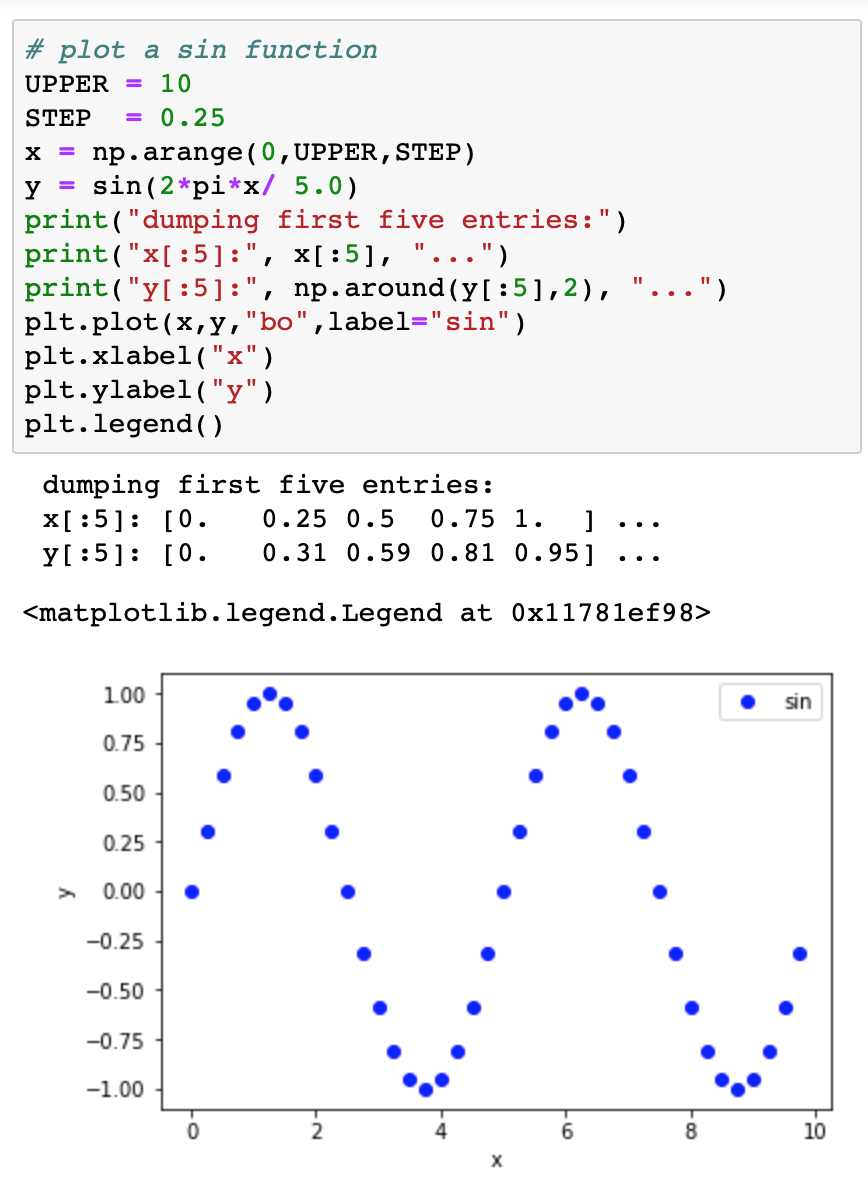
\includegraphics[width=0.65\textwidth]{figs//plotting/plotting.png} 
\caption{Circuit for verifying Ohm's law as a (a) circuit diagram, and (b) implemented using your lab equipment.}
\label{fig:plotsin}
\end{center}
\end{figure}

Consider the Jupyter notebook example in Fig.~\ref{fig:plotsin} which
plots a sine function sampled at discrete values.  Note the following
key features, which you will use repeatedly today and in future labs:
\begin{itemize}
\item Use of global variables {\tt UPPER} and {\tt STEP} at the top of
  the snippet, allowing for easy adjustment of parameters that affect
  the plot.
\item Use of {\tt np.arange} to define an array of x values.
\item Creation of the array y, defined by $y = \sin(2\pi x / 5)$ for each value of x.  One of the great joys of using numpy is the ability to avoid getting bogged down with explicit for loops.
\item Use of slicing techniques {\tt x[:5]} to show only the first five entries for debugging.  
\item Plotting the arrays of $x$ and $y$ values with {\tt plt.plot}  using the {\tt "bo"} option for blue circles.
\item Defining appropriate axis labels with {\tt plt.xlabel} and {\tt plt.xlabel}. 
\item Creation of a legend using the {\tt label} option to {\tt plt.plot} and the {plot.legend()} command.
\end{itemize}
Notice that even in this simple example, I've added some intermediate
feedback from my code in the form of the screen dumps of the first few
values of $x$ and $y$.  It's a common pitfall to try and rush ahead to
the final product when programming.  But it is much faster and
reliable to break your task into small steps, and establish feedback
at each small step.  To plot a continuous function with Scientific
Python, you will still use discrete data but:

\begin{itemize}
 \item Use much finer binning of the $x$-axis variable to draw a smooth curve. 
 \item Use the line option {\tt "-"} or dashed line {\tt "--"} instead of points with {\tt "o"}. 
\end{itemize} 

\noindent
{\bf Plot 1:}  Plot the quadratic function $y = x^2$ with the following requirements:
\begin{itemize}
 \item Plot in the range $x = [0,20)$.
 \item Plot discrete samples with a step size of $2$ using blue circles.
 \item On the same axis, plot the corresponding smooth function using a red solid line.
 \item Add appropriate axis labels. 
 \item Add a legend for the ``discrete'' and the ``smooth''  function.
\end{itemize}

\section{Multivariate analysis using boolean masks}
\begin{figure}[htbp]
\begin{center}
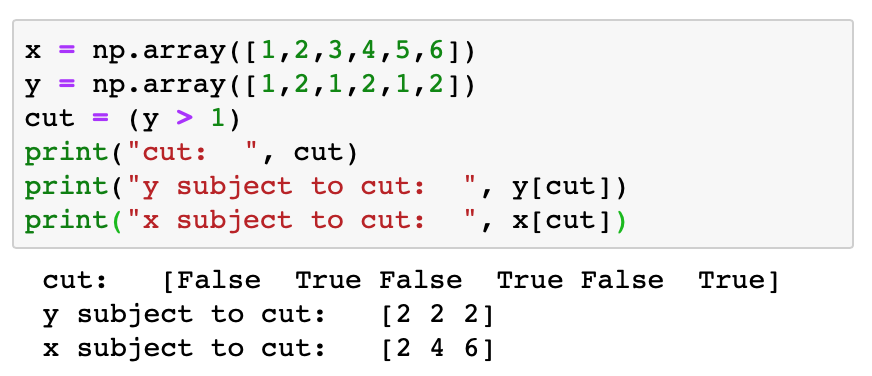
\includegraphics[width=0.65\textwidth]{figs//plotting/booleanmasks.png} 
\caption{Using boolean masks to cut on variable $y$.}
\label{fig:booleanmasks}
\end{center}
\end{figure}

A powerful technique in Scientific Python for performing analysis involving multiple variables uses boolean masks as shown in Fig.~\ref{fig:booleanmasks}.  In the example:
\begin{itemize}
\item Two numpy arrays $x$ and $y$ {\tt of the same length} are defined to contain the collected data.
\item The cut defined by $y > 1$ is a boolean array of the same length as $x$ and $y$ which is true at indices where the condition is met and false where it is not.
\item The subset of the entire $y$ array defined by {\tt y[cut]} consists only of those entries of $y$ for which the condition $y>1$ is met.
\item The subset of the entire $x$ array defined by {\tt x[cut]} consists only of those entries of $x$ for which the condition $y>1$ is met for the corresponding y value.
\end{itemize}
The last item shows the real power of this technique, one can look at one variable subject to constraints on another variable.

\begin{table}
\caption{Sample data for a voltage measurement subject to high frequency noise.}
\label{tbl:hfnoiseeg}
\begin{center}
\begin{tabular}{lll}
$t~(\rm s)$ & $v~(\rm V)$ & $n$ \\
0.4  & 0.25  &  2.8 \\
1.1  & 2.37  &  7.3 \\
1.4  & 1.69  &  9.7 \\
1.9  & 0.93  &  1.3 \\
2.5  & -1.0  &  6.2 \\
3.0  & 0.95  &  4.8 \\
3.4  & 1.22  &  6.9 \\
4.1  & 0.54  &  4.0 \\
4.4  & 0.37  &  1.9 \\
4.8  & 0.13  &  4.0 \\
5.5  & -2.04  &  9.5 \\
6.2  & -2.06  &  8.7 \\
6.5  & -0.81  &  2.3 \\
7.0  & -0.95  &  5.3 \\
7.5  & 0.98  &  9.7 \\
7.9  & 0.27  &  8.3 \\
8.5  & -0.81  &  0.1 \\
9.0  & -0.59  &  5.1 \\
9.4  & -0.37  &  4.4 \\
9.9  & 0.56  &  9.9 \\
\end{tabular}
\end{center}
\end{table}

Next consider the sample data in Table~\ref{tbl:hfnoiseeg} which comes from experimental measurements of a voltage level $v$ at discrete times $t$.  The measurement is subject to a high-frequency noise monitoring by the variable $n$.  The noise is only present for $n > 6.0$.  A straightforward way to load this data into scientific python is by defining numpy arrays for each variable as follows:
\begin{verbatim}
t = np.array([0.4, 1.1, 1.4, 1.9, 2.5, 3.0, 3.4, 4.1, 4.4, 4.8, 
                     5.5, 6.2, 6.5, 7.0, 7.5, 7.9, 8.5, 9.0, 9.4, 9.9])
v = np.array([ 0.25, 2.37, 1.69, 0.93, -1.0, 0.95, 1.22,   
                      0.54, 0.37, 0.13, -2.04, -2.06, -0.81, -0.95,  
                      0.98, 0.27, -0.81, -0.59, -0.37, 0.56])
n = np.array([2.8, 7.3, 9.7, 1.3, 6.2, 4.8, 6.9, 4.0, 1.9, 4.0,  
                      9.5, 8.7, 2.3, 5.3, 9.7, 8.3, 0.1, 5.1, 4.4, 9.9])
\end{verbatim}

\noindent
{\bf Plot 2} Prepare a plot of the sample data subject to the following:
\begin{itemize}
 \item Plot the voltage as a function of time as discrete data using red points.
 \item Define the boolean array {\tt keep} based on the noise reducing condition $n<=6.0$.
 \item Plot the voltage as a function of time, subject to the noise reducing condition using blue points.
 \item Plot the function $\sin(2 \pi x / 10)$ as a smooth function.
 \item Add appropriate axis labels.
 \item Add a legend for ``raw'' data with no cut, ``clean'' data with noise removed, and your continuous ``sin'' function.   
\end{itemize}
Your plot will reveal a clear sine function in the discrete data (after noise removal) consistent with the continuous function.  





\chapter{DC Circuits}

\section{Introduction}

In this lab, you will learn how to use your digital multimeter (DMM) and bench-top DC power supply to explore DC circuits involving resistors.  You will experimentally verify Ohm's law and the equivalent resistance for resistors in series and parallel.  You will solder two resistor circuits to explore the $\Delta$-$Y$ transformation for three terminal networks.

\section{Benchtop Power Supply}
% MASTECH HY3005F-3

\section{Digital Multimeter}
% Triplett 9007 (often blown fuse)
% Mastech MS8264 (resettable fuse)

\begin{figure}[htbp]
\begin{center}
\begin{tabular}{c@{\hskip 2cm}c}

\begin{circuitikz}[line width=1pt]
\draw (0,0) to[battery1,bipoles/length=1.5cm] ++(0,+4.0) to[short] ++(2.0,0) coordinate(A);
\draw (A) to[resistor,l_=$R_1$] ++(0,-2.0) to[short] ++(0,-2.0) to[short] ++(-2,0);
%node[ground,yscale=2.0]{};
\draw (0,1.7) node[left]{$-$};
\draw (0,2.4) node[left]{$+$};
\draw (A) to[short,*-] ++(2.0,0.0) to[short] ++(0.0,-1.0) node[component]{V} to[short] ++(0.0,-1.0) to[short,-*] ++(-2.0,0);
\end{circuitikz} &

\begin{circuitikz}[line width=1pt]
\draw (0,0) to[battery1,bipoles/length=1.5cm] ++(0,+4.0) to[short] ++(2.0,0);
\draw (A) to[resistor,l_=$R_1$] ++(0,-2.0) to[short] ++(0,-1.0) 
node[component]{A} to[short] ++(0,-1.0) to[short] ++(-2.0,0);
%node[ground,yscale=2.0]{};
\draw (0,1.7) node[left]{$-$};
\draw (0,2.4) node[left]{$+$};
\end{circuitikz} \\

(a) & (b) \\
\end{tabular}
\caption{Circuits for verifying Ohm's law.}
\label{fig:dmmscematic}
\end{center}
\end{figure}




% Triplett 9007 (often blown fuse)
% Mastech MS8264 (resettable fuse)
% Wish Board No.  206
% MASTECH HY3005F-3

In this lab, you will use two new pieces of lab equipment:  your bench-top power supply and your digital multimeter (DMM).

Your bench-top supply provides up to XX volts of DC power on two independent channels.  For this lab, we'll only be using a single channel.  Each supply has two associated knobs, one controlling the maximum allowed current, and one controlling the maximum voltage.  The supply will provide the maximum voltage subject to those constraints.  Usually your are primarily concerned with setting the voltage by the voltage knob, but it is a good habit, which will save you from losing components, to set the current as low as possible.  An LED indicates if your circuit is current limited or voltage limited.  You can adjust the current limit until just beyond the point where your circuit become voltage limited.

The supply is floating, it provides the specified voltage between the black and red outputs without referencing either to ground.  If you want to provide a ground referenced voltage you explicitly connect the green output to the red (positive) terminal or the black (negative) terminal.

(Discuss limits)

Your DMM can measure voltage, resistance, and current.






\section{Verification of Ohm's Law}

\begin{figure}[htbp]
\begin{center}
\begin{tabular}{c@{\hskip 2cm}c}

\begin{circuitikz}[line width=1pt]
\draw (0,0) to[battery1,bipoles/length=1.5cm] ++(0,+4.0) to[short] ++(2.0,0) coordinate(A);

\draw (A) to[resistor,l_=$R_1$] ++(0,-2.0) to[short] ++(0,-1.0) 
node[component]{A} to[short] ++(0,-1.0) to[short] ++(-2.0,0);
%node[ground,yscale=2.0]{};
\draw (0,1.7) node[left]{$-$};
\draw (0,2.4) node[left]{$+$};
\draw (A) to[short,*-] ++(2.0,0.0) to[short] ++(0.0,-1.0) node[component]{V} to[short] ++(0.0,-1.0) to[short,-*] ++(-2.0,0);
\end{circuitikz} &
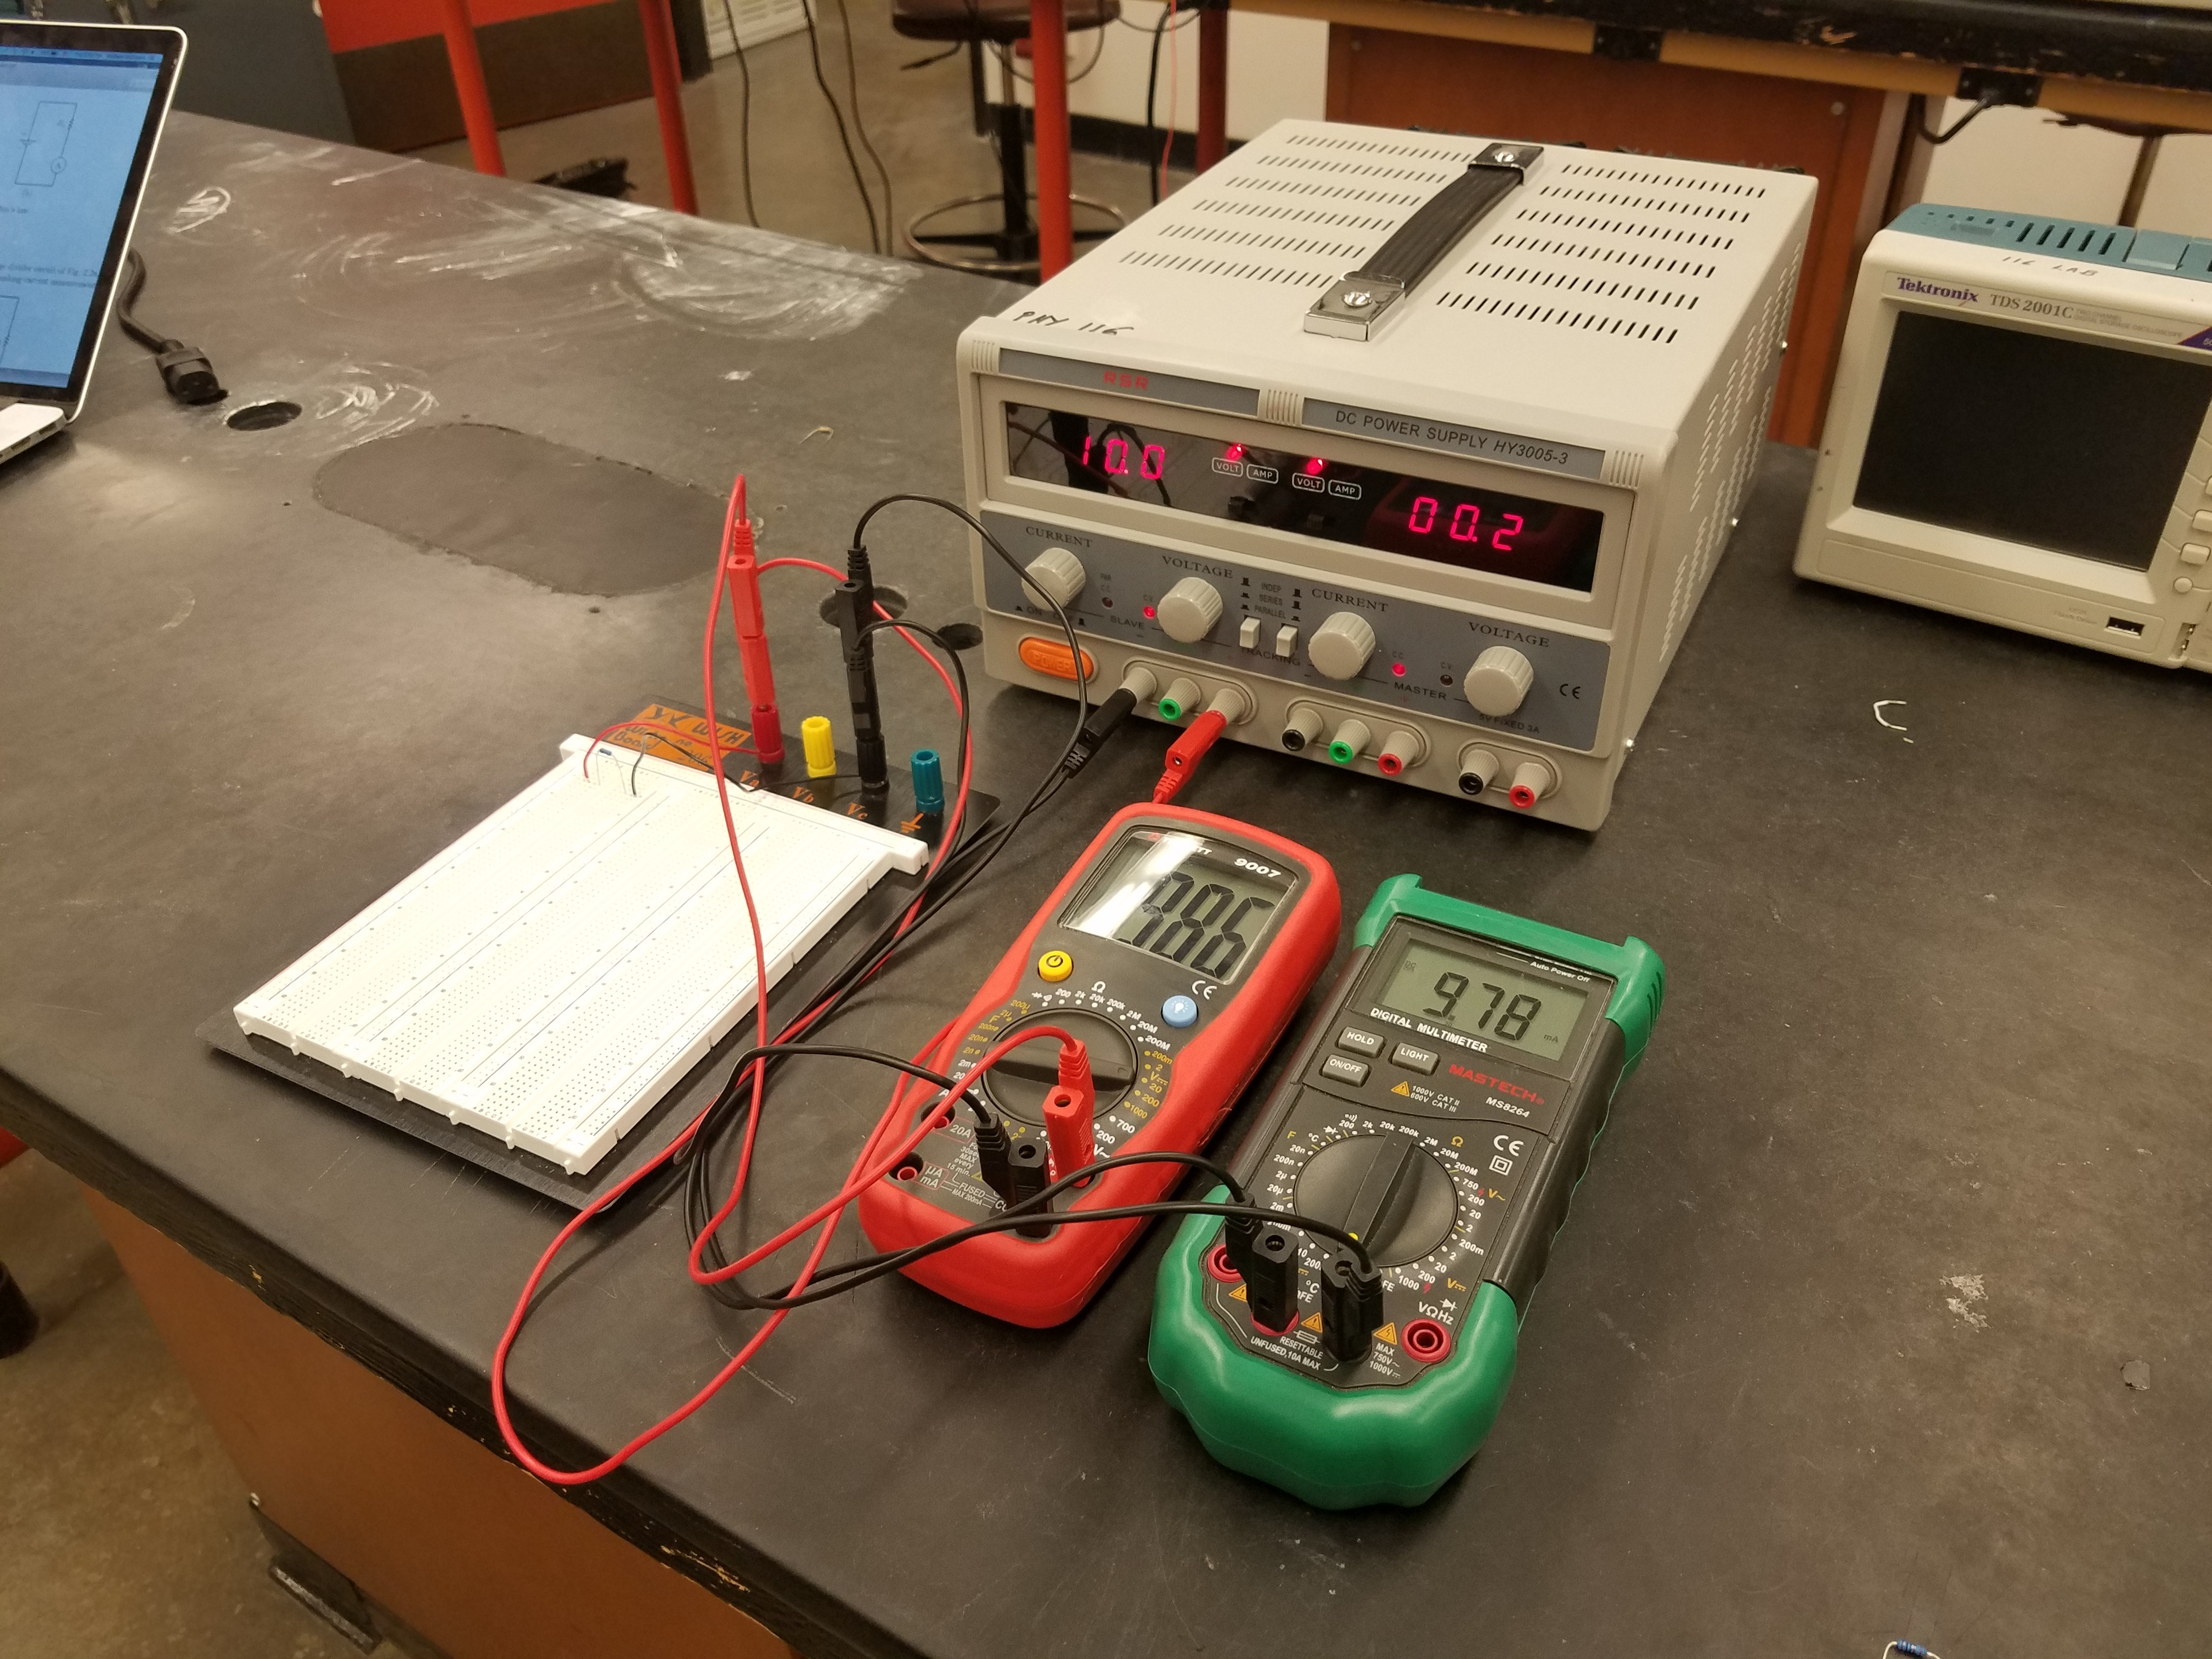
\includegraphics[height=0.25\textheight]{figs/labs/dc_circuits/setup.jpg} \\
(a) & (b) \\
\end{tabular}
\caption{Circuit for verifying Ohm's law as a (a) circuit diagram, and (b) implemented using your lab equipment.}
\label{fig:ohmslaw}
\end{center}
\end{figure}


Build the circuit in Fig.~\ref{fig:ohmslaw}.  Use a resistor $R_1 = 1.0~{\rm k\Omega}$ with a $1\%$ tolerance.  Use your Triplett 9007 as the voltmeter and the Mastech MS8624 as the current meter.  Use your benchtop power supply to provide the voltage.  

By adjusting the voltage setting of the power supply, take a series of voltage and current measurements with voltage across the resistor at target voltages from $1$ to $10~\rm V$ in steps of $1~\rm V$.   Generally, you can measure more precisely than you can control, so never fuss about trying to measure the voltage at exactly the target value, instead, simply record e.g. $V=1.04~\rm V$ along with your current measurement and move on to the next target value.

While recording data, check that the current values you measure are consistent with what you expect given the voltage across the resistor and resistance.  You should {\em always} make quick sanity calculations when collecting data, otherwise you risk wasting time collecting useless data!

{\bf Plot 1:}  Plot the current versus voltage of your ten data points (using option {\tt "o"}).  Draw a line (using option {\tt "-"}) for the current versus voltage curve of a $1.0~\rm k\Omega$ resistor.  Make certain your plot has appropriate axis labels, including appropriate units in parenthesis, and a legend distinguishing data from your expectation (``expected").  {\bf Measurement 1:}  After taking your last measurement, leave all the connections in place and the power-supply at $10~\rm V$.  Record in your log book the resistance of the resistor $R_1$ reported by your DMM.  Is this a reasonable measurement?  {\bf Measurement 2:}  Turn off the DC supply and record the resistance reported by the DMM.  Is this accurate?  {\bf Measurement 3:}  Remove the resistor from your circuit and measure the resistance with your DMM.  Is this accurate?

\begin{figure}[htbp]
\begin{center}
\begin{tabular}{c@{\hskip 2cm}c}

\begin{circuitikz}[line width=1pt]
\draw (0,0) to[battery1,bipoles/length=1.5cm] ++(0,+4.0) to[short] ++(2.0,0) coordinate(A);
\draw (A) to[resistor,l_=$R_1$] ++(0,-2.0) to[short] ++(0,-2.0) to[short] ++(-2,0);
%node[ground,yscale=2.0]{};
\draw (0,1.7) node[left]{$-$};
\draw (0,2.4) node[left]{$+$};
\draw (A) to[short,*-] ++(2.0,0.0) to[short] ++(0.0,-1.0) node[component]{V} to[short] ++(0.0,-1.0) to[short,-*] ++(-2.0,0);
\end{circuitikz} &

\begin{circuitikz}[line width=1pt]
\draw (0,0) to[battery1,bipoles/length=1.5cm] ++(0,+4.0) to[short] ++(2.0,0);
\draw (A) to[resistor,l_=$R_1$] ++(0,-2.0) to[short] ++(0,-1.0) 
node[component]{A} to[short] ++(0,-1.0) to[short] ++(-2.0,0);
%node[ground,yscale=2.0]{};
\draw (0,1.7) node[left]{$-$};
\draw (0,2.4) node[left]{$+$};
\end{circuitikz} \\
(a) & (b) \\
\end{tabular}
\caption{Circuits for verifying Ohm's law.}
\label{fig:missing}
\end{center}
\end{figure}


\section{Voltage Divider}
One circuit you will encounter again and again is the humble voltage divider circuit of Fig.~\ref{fig:dividers}a.  Modify your setup to include an additional resistor $R_2 = 4.7~\rm k\Omega$ in series with your resistor $R_1 = ~\rm 1~\rm k\Omega$.  Before installing it in your circuit, record the actual value of your resistor $R_2$ in your log book.

{\bf Measurement 4:} adjust the supply voltage to $10~\rm V$ and record the voltage across resistor $R_1$, the voltage across resistor $R_2$, and the current through the divider.  Compare these measured values to your expectation.

Now adjust your circuit so that $R_1$ and $R_2$ are in parallel and set the supply to $10~\rm V$  {\bf Measurement 5:}  Record the voltage across the resistors $R_1$ and $R_2$ and the total current through both resistors.  Compare the measured current to your expectation.

\begin{figure}[htbp]
\begin{center}
\begin{tabular}{c@{\hskip 2cm}c}
\begin{circuitikz}[line width=1pt]
\draw (0,0) to[battery1,bipoles/length=1.5cm] ++(0,+4.0) to[short] ++(2.0,0);
\draw (A) to[resistor,l_=$R_1$] ++(0,-2.0) to[resistor,l_=$R_2$] ++(0,-2.0) to[short] ++(-2.0,0);
%node[ground,yscale=2.0]{};
\draw (0,1.7) node[left]{$-$};
\draw (0,2.4) node[left]{$+$};
\end{circuitikz} &
\begin{circuitikz}[line width=1pt]
\draw (0,0) to[battery1,bipoles/length=1.5cm] ++(0,+4.0) to[short] ++(2.0,0) coordinate(A);
\draw (A) to[resistor,l_=$R_1$] ++(0,-4.0) to[short] ++(-2,0);
%node[ground,yscale=2.0]{};
\draw (0,1.7) node[left]{$-$};
\draw (0,2.4) node[left]{$+$};
\draw (A) to[short,*-] ++(2.0,0.0) to[resistor,l_=$R_2$] ++(0.0,-4.0) to[short,-*] ++(-2.0,0);
\end{circuitikz} \\
(a) & (b) \\
\end{tabular}
\caption{Circuits for driving an LED (a) directly from the signal voltage and (b) using a diode switch.}
\label{fig:dividers}
\end{center}
\end{figure}


\section{$\Delta$-$Y$ transformation}

Consider the two different circuits shown in Fig.~\ref{fig:deltay}.  If we are willing to neglect the central vertex in the left hand circuit, the two circuits are equivalent in the case that $R_1 = R_2 / 3$.   Using your soldering iron, 




\begin{figure}[htbp]
\begin{center}
\begin{tabular}{c@{\hskip 2cm}c}
\begin{circuitikz}[line width=1pt]
\draw (0,0) coordinate(A);
\draw (A) to[R,l_=$R_1$,*-*] ++(0,2.0);
\draw (A) to[R,*-*] ++(-1.73,-1);
\draw (A) to[R,*-*] ++(1.73,-1);
\draw (-0.5,0) node[left]{$R_1$};
\draw (1.25,0) node[left]{$R_1$};

\end{circuitikz} &
\begin{circuitikz}[line width=1pt]
\draw (0,2) to [R] (1.73,-1) to [R,*-,l_=$R_2$] (-1.73,-1) to [R,*-*] (0,2);
\end{circuitikz} \\
(a) & (b) \\
\end{tabular}
\caption{Equivalent three-node circuits.}
\label{fig:deltay}
\end{center}
\end{figure}


\section{Additions}

Effect of resistance measurement with current in resistor?

Loading of circuit by DMM.



\chapter{Equivalent Circuits}

In this lab, you will explore Thevenin equivalent circuits. You will
also solder two resistor circuits to explore the $\Delta$-$Y$
transformation for three terminal networks. For this lab, both logbook
and Jupyter Notebook entries are required. You can find the resistors
inside storage cabinet at the table to your left and cables hanging at
the wall to your left. Please return them at the end of the lab.

\section{Calculations}

\noindent
During lecture we determined an equation for the Thevenin
equivalent voltage $V_{\rm th}$ and resistance $R_{\rm th}$ from the
values $V_1, V_2, R_1, R_2, R_3$ for the circuit shown in
Fig.~\ref{fig:thevenin}.
%Hint: Use the superposition principle. Find the equivalent resistance
%by setting the voltage $V_1$ and $V_2$ to zero, i.e. shorting them in
%the circuit.  Then calculate two contributions to the Thevenin
%voltage, one with $V_1$ set to zero and one with $V_2$ set to zero.
%The actual Thevenin voltage is the sum of these two contributions.
%Play close attention to the polarity of $V_2$ as drawn, i.e. that a
%positive value of $V_2$ tends to make the voltage $V_{\rm a b}$
%negative.

\begin{measurement} 
Repeat this calculation in terms of $V_1, V_2, R_1, R_2, R_3$ in your
logbook together with the sketch of the circuit.
\end{measurement}

\begin{figure}[htbp]
\begin{center}
\begin{tabular}{c@{\hskip 2cm}c}
\begin{circuitikz}[line width=1pt]
\draw (0,0) to[voltage source,bipoles/length=1.5cm,l=$V_1$,invert] ++(0,2.0)
coordinate(X) to[R,l=$R_3$,-*] ++(2.0,0); \draw (X) to[R,l=$R_1$]
++(0,2.0) to[short,-*] ++ (2.0,0) coordinate(X) to[short,-o] ++
(1.0,0) node[right]{B}; \draw (X) to[voltage
  source,bipoles/length=1.5cm, l=$V_2$,invert] ++(0,-2.0) to[R,l=$R_2$]
++(0,-2.0) coordinate(X) to[short,*-o] ++ (1.0,0) node[right]{A};
\draw(X) to[short] ++(-2.0,0);
\end{circuitikz} &
\begin{circuitikz}[line width=1pt]
\draw (0,0) coordinate(X) to[voltage source,bipoles/length=1.5cm,l=$V_{\rm th}$,invert] ++(0,2.0) to[R,l=$R_{\rm th}$,-*] ++(0,2.0)
to[short,-o] ++ (3.0,0) node[right]{B};
\draw(X) to[short,-o] ++ (3.0,0) node[right]{A};
\end{circuitikz} \\
(a) & (b) \\
\end{tabular}
\caption{The circuit (a) you will be building in lab and it's (b) Thevenin Equilvalent.}
\label{fig:thevenin}
\end{center}
\end{figure}

\section{Thevenin Equivalent Circuit}

Build the circuit (on a breadboard) in Fig.~\ref{fig:thevenin} using $R_1 = 3.3~\rm
k\Omega$, $R_2 = 3.9~\rm k\Omega$, and $R_3 = 4.7~\rm k\Omega$.
Supply $V_1 = 10~\rm V$ and $V_2 = 5~\rm V$ using your two channel
bench-top power supply.  In the diagram, the supplies are not
referenced to ground or each other, so make certain that your supply
is set to provide independent outputs and do not add any jumpers to
ground.  Take careful note of the polarity of the supplies, so
e.g. the negative (black) output of $V_1$ is connected to point (A)
whereas the negative (black) output of $V_2$ is connected to point
(B).Use your Triplett 9007 as a voltmeter and the Mastech MS8624 as a
current meter.   

\begin{measurement} 
Compute $V_{\rm th}$, $R_{\rm th}$, and the short-circuit current
$I_{\rm sc}$ for the particular values of $R_1$,$R_2$,$R_3$,$V_1$, and
$V_2$ you will be using in the lab. Record these values in your logbook.  
\end{measurement}

\begin{measurement} 
First measure the open circuit voltage $V_{\rm ab}$.  Next short the
points (a) and (b) through your current meter. Record these values in
your logbook.  These values should closely match the Thevenin voltage
and short-circuit current which you have already calculated.  If not,
you should check your work and find the discrepancy before
proceeding. Record your comments in the logbook.
\end{measurement}

\begin{measurement}  
Next you will measure the voltage across and current through a load
resistor connected between the terminals at (A) and (B) to
experimentally determine the IV curve for your circuit.  Recall from
the previous lab that you measure the current by connecting your meter
in series and the voltage by connecting your meter in parallel.  As
before, use your Triplett 9007 as a voltmeter and the Mastech MS8624
as a current meter. Make simultaneous current and voltage measurements
for three different values of the load resistance $R = 470~{\rm
  \Omega}, 1.2~\rm k\Omega, 4.7~\rm k\Omega.$ Record these values in
your logbook.
\end{measurement}

\section{Analysis}

\begin{plot}
To present your analysis you should produce a plot similar to that of
Fig.~\ref{fig:egthev}.  Your plot should show the Thevenin equivalent
source IV curve for the circuit you built in lab.  You should also
draw theoretical load IV curves for the three resistor values you used
to make current and voltage.  Finally, you should include data points
for the five current and voltage measurements which you have made.
\end{plot}

\begin{figure}[htbp]
\begin{center}
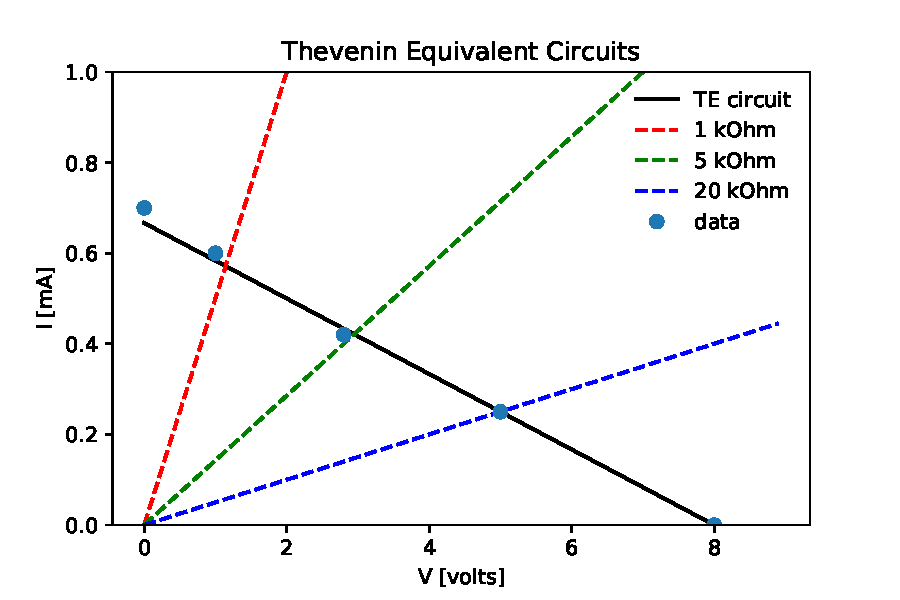
\includegraphics[width=0.75\textwidth]{figs/labs/thevenin/final.pdf} 
\caption{Example of IV curves for Thevenin equivalent source circuit with various load resistors. }
\label{fig:egthev}
\end{center}
\end{figure}

\section{Impact of the Multimeter on the Measured Circuit}

A perfect DMM would not affect the circuit you are measuring at all,
but this is not the case in practice. An ideal voltmeter has infinite
resistance so that it draws zero current when measuring voltage across
two points. An ideal ammeter has zero resistance so that there is no
voltage change as the current passes through it.  Your DMM has a small
non-zero resistance when used as an ammeter, and a large resistance
when used as a voltmeter.

\begin{measurement} 
Build the voltage divider of Fig.~\ref{fig:dividers}a but with
$V_1=10~\rm{V}$ and $R_1 = R_2 = 10~\rm{M\Omega}$. Record the voltage
across one of the resistors. Compare the value your measure with what
you predict for a perfect DMM. Sketch the circuit with a realistic DMM
and calculate the resistance of your DMM when used as a voltmeter.
\end{measurement}

\noindent
This is a \textbf{sign-off point} for this lab. 

\section{$\Delta-Y$ Transformation}

Not everyone will complete this portion of the lab.  Do your best to
finish as much as you can.

\begin{figure}[htbp]
\begin{center}
\begin{tabular}{c@{\hskip 2cm}c}
\begin{circuitikz}[line width=1pt]
\draw (0,0) coordinate(A);
\draw (A) to[R,l_=$R_A$,*-*] ++(0,2.0) node[above]{A};
\draw (A) to[R,*-*] ++(-1.73,-1) node[left]{B};
\draw (A) to[R,*-*] ++(1.73,-1) node[right]{C};
\draw (-0.5,0) node[left]{$R_B$};
\draw (1.25,0) node[left]{$R_C$};

\end{circuitikz} &
\begin{circuitikz}[line width=1pt]
\draw (0,2) to [R] (1.73,-1) node[right]{C} to [R,*-,l_=$R_{BC}$] (-1.73,-1) node[left]{B} to [R,*-*] (0,2) node[above]{A};
\draw (-0.75,1) node[left]{$R_{AB}$};
\draw (0.8,1) node[right]{$R_{AC}$};
\end{circuitikz} \\
(a) & (b) \\
\end{tabular}
\caption{Equivalent three-node circuits.}
\label{fig:deltay}
\end{center}
\end{figure}

Consider the two different networks shown in Fig.~\ref{fig:deltay}.
If there are no external connections to the central node in the
left-hand circuit, the two networks are equivalent if:
\begin{displaymath}
R_{A} = \frac{R_{AC} R_{AB}}{R_{AB} + R_{AC} + R_{BC}}
\end{displaymath}
as well as two similar equations for $R_{B}$ and $R_{C}$.  Going in the other direction we have:
\begin{displaymath}
R_{AB} = \frac{R_{A}R_{B} + R_{A}R_{C} + R_{B}R_{C}}{R_{C}}.
\end{displaymath}
These transformations are more general than the series and parallel
laws, which you can derive by considering the case that $R_{BC}=0$ for
parallel resistors, and $R_{C} \to \infty$ for series resistors.  They
allow one to simplify more complicated networks for which the series and
parallel equivalence relations are insufficient.

In the special case that $R_{A} = R_{B} = R_{C} = R$ it follows that 
\begin{displaymath}
R_{AB} = R_{AC} = R_{BC} = 3 R.
\end{displaymath}

Use your soldering iron to construct the left-hand network using
$R_{A} = R_{B} = R_{C} = 1~\rm k\Omega$.  Then construct the
equivalent right-hand network using $R_{AB} = R_{AC} = R_{BC} =
3.0~\rm k\Omega$.  If $3~\rm k\Omega$ resistors are not available, you
can construct one by using a $33~\rm k\Omega$ in parallel with a
$3.3~\rm k\Omega$ resistor.

Make sure the soldering iron is on, and the sponge is moist.  There is
one soldering iron per two workstation. Find the squeeze bottle around
the lab. The clamps (possibly various styles) are on the shelves to
your left. Twist the leads of the resistor together to make initial
connections, then hold the arrangement securely in the clamp.  Wipe
the tip of the hot iron on the sponge to clean it, then apply a small
amount of solder to the tip by touching the hot iron to the solder
wire.

Heat the connection by holding the soldering iron against it, then
bring the solder wire in contact with the heated connection (not the
soldering iron) You want the iron to heat the connection, and then the
connection to melt and draw in the solder.  The little bit of solder
on the tip is only there to ensure good thermal conduct between the
tip and the connection: don't ``paint'' the solder onto the
connection.

\begin{measurement} 
Check the resistance between pairs of terminals on your creations, and
compare with your expectation. Record those values in your logbook. You can bring your creations home if
you like or bring them to the front desk. 
\end{measurement}

This is an additional \textbf{sign-off point} for this lab. 

\noindent
Please return all the components you took and cables to their place. Leave you workstation clean. 


\chapter{Alternating Current and Time Varying Signals}

\section{Introduction}

In this lab you will use two essential new pieces of lab equipment:
the digital oscilloscope and the function generator.  You will learn
how to measure AC voltages with your DMM, how to trigger on and view
time-dependent wave forms on your digital oscilloscope.  You will
produce Lissajous figures on your oscilloscope and reproduce them
using Scientific Python.  For this lab there are both logbook and
Jupyter notebook entries.

\section{Function Generator}

This section introduces you to your Function Generator and illustrates
some of the common used features and pitfalls.  It should not take
more than about one-half hour to complete.

Connect the output of Channel 1 directly to the Voltage measurement
input of your Triplett 9007 DMM, using a coaxial cable with BNC
connectors, and a BNC to banana plug adapter as shown in
Fig.~\ref{fig:dmm_setup}.  BNC is a type of quick connector often used
for coaxial cable.  Coaxial cable is a type of electrical cable that
can transmit high frequency signals with low losses. It has an inner
conductor surrounded by an insulating layer, surrounded by a
conducting shield.  Coaxial cable has a characteristic impedance,
which specifies the resistance that should be placed at the receiving
end of the cable to minimize reflections, which can degrade high
frequency signals.  Your coaxial cable has a characteristic impedance
of $50~\rm \Omega$.

\begin{figure}[htbp]
\begin{center}
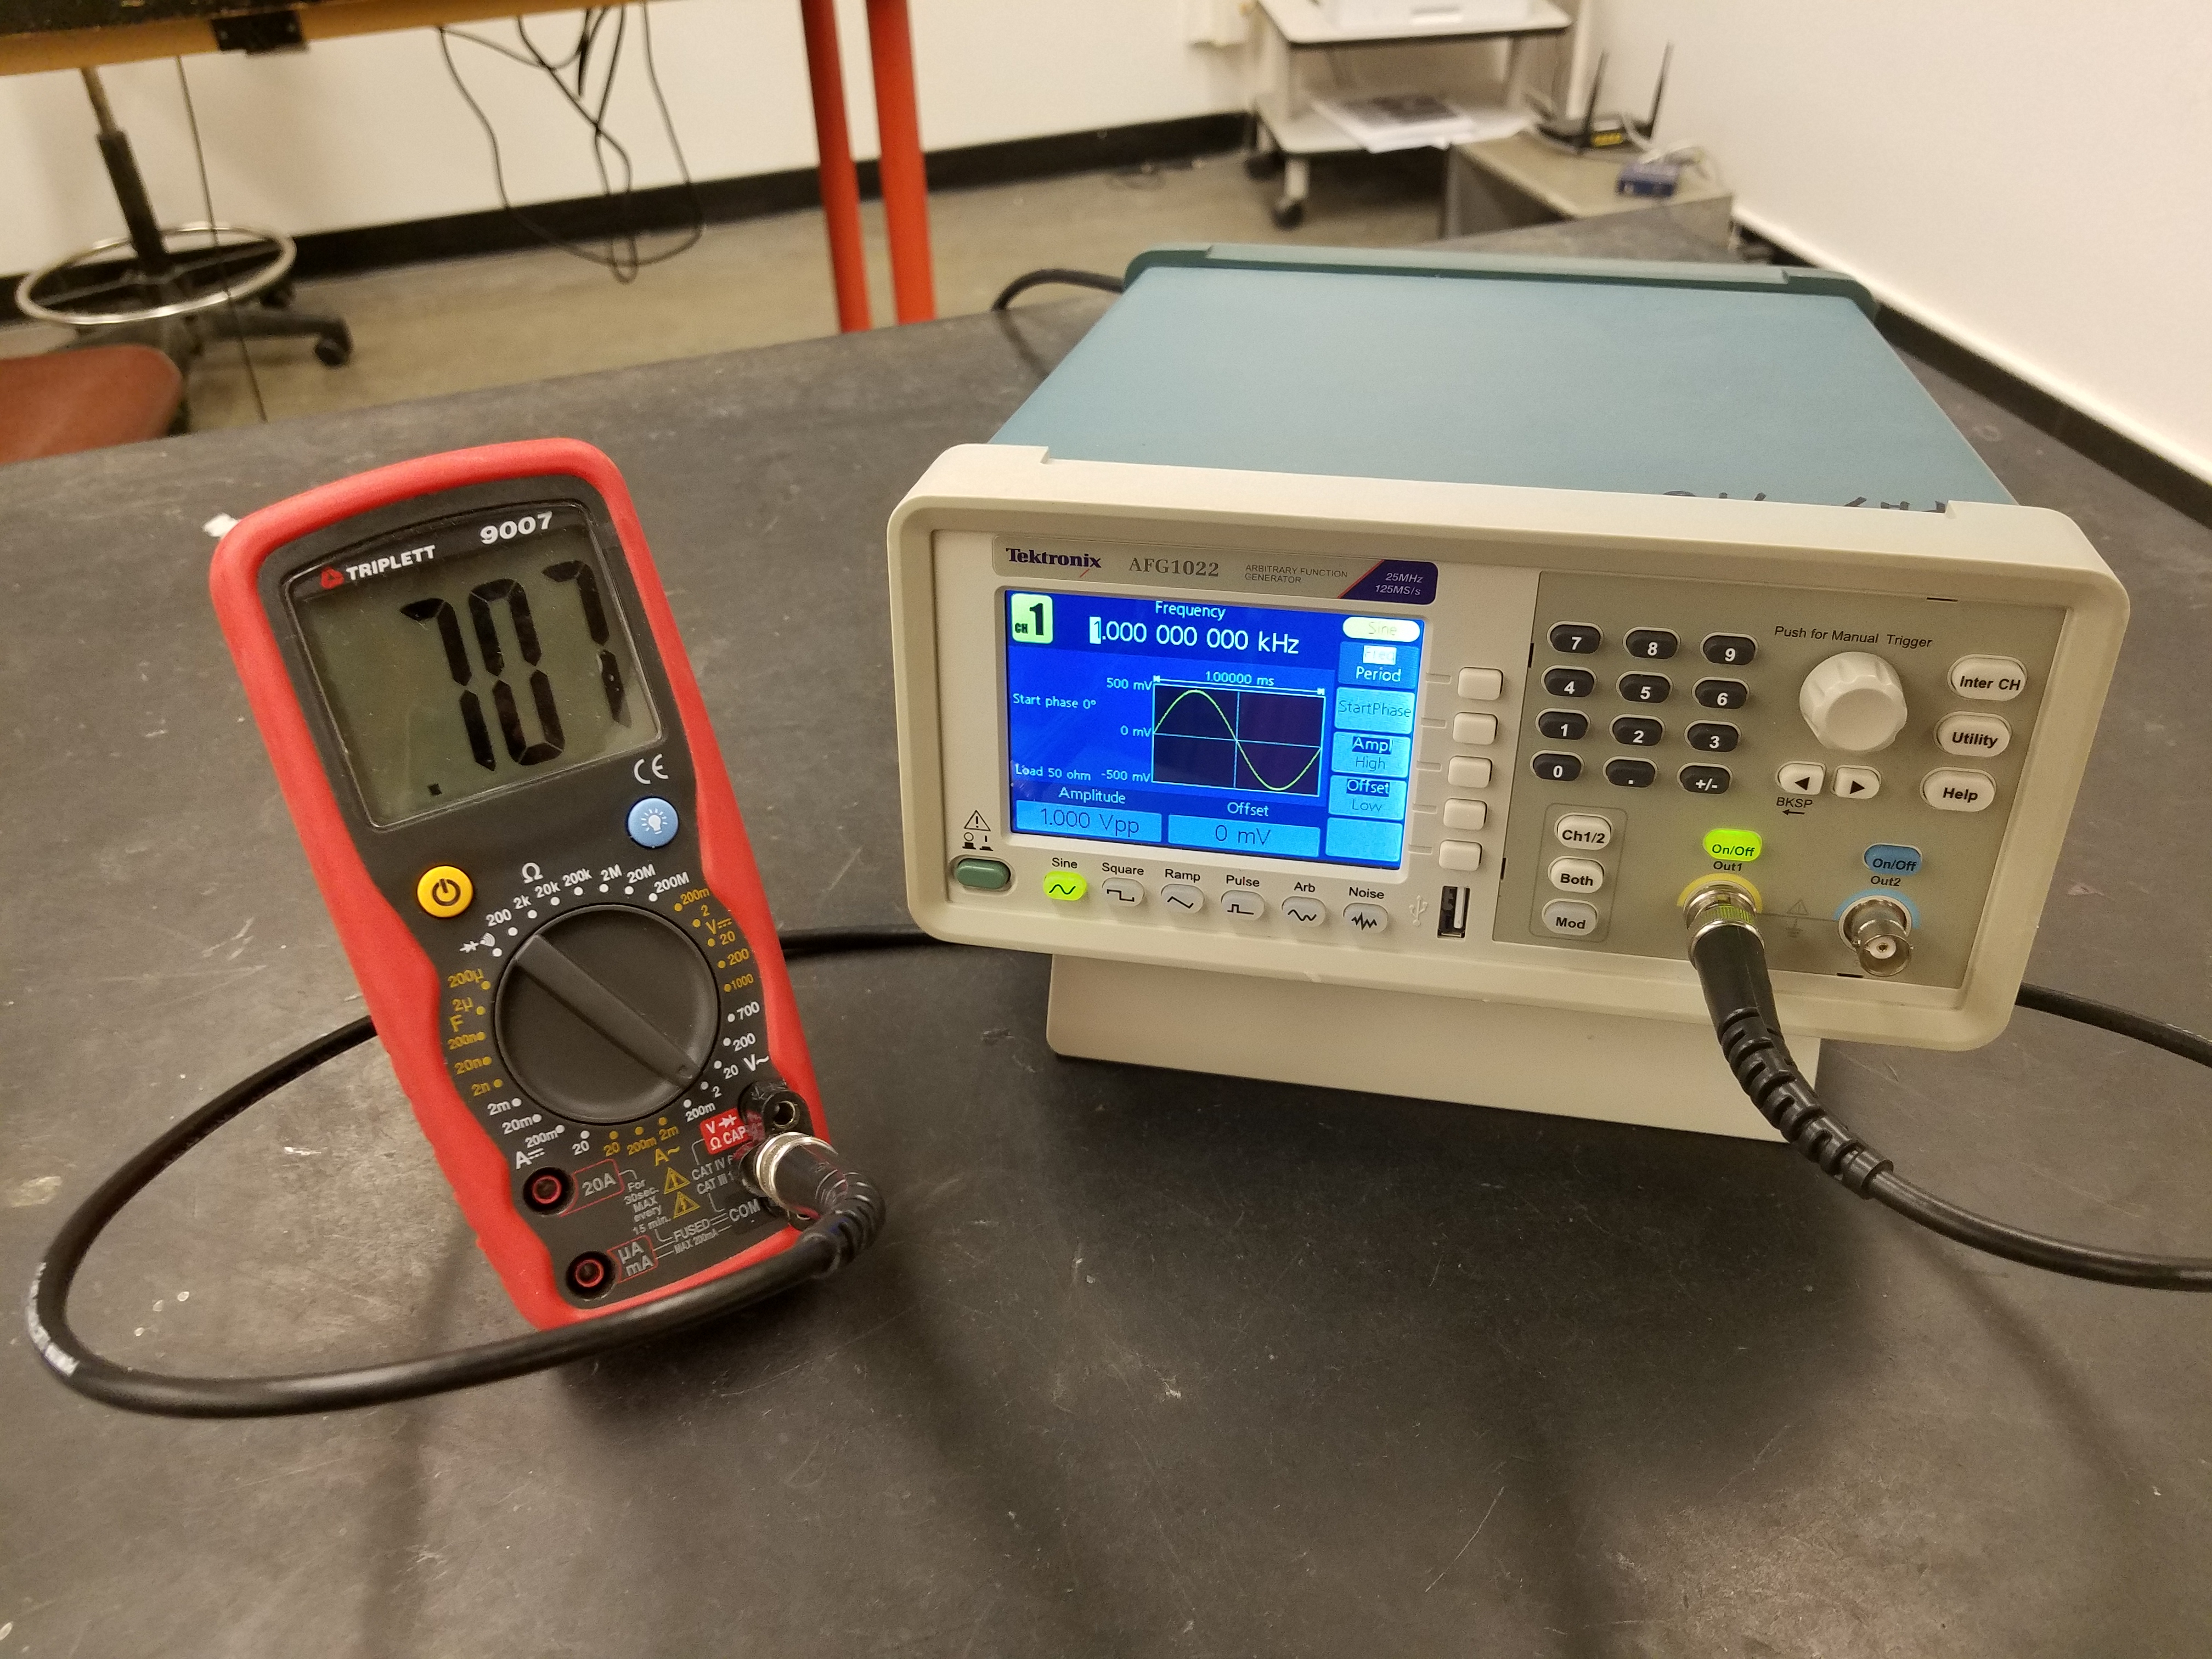
\includegraphics[width=0.45\textwidth]{figs/labs/lissajous/generator_dmm_setup.jpg} 
\caption{Connect the Channel 1 Output of your function generator directly to your DMM.}
\label{fig:dmm_setup}
\end{center}
\end{figure}

Turn on power to the function generator.  Then set your function
generator to the factory default:
\begin{displaymath}
\rm Utility\;Button \to System \to Set\;to\;Default \to Select.
\end{displaymath}
You must perform this step today for the instructions that follow to
make sense.  With shared equipment, it is essential to know how to
restore the factory default, in case another user has left the device
with strange settings.  You don't need to start with this step every
lab, but it is a fast way to recover when you encounter strange
behavior in your equipment.

The factory default settings are set to produce a Sine function with a
peak-to-peak voltage $v_{\rm pp} = 1.0~\rm V$ and a frequency $f=1~\rm
kHz$.  We'll leave that as is for now.  To turn on the output, push
the ``On/Off'' directly above the coaxial output for Channel 1, and
then ensure that the button is lit.

\begin{figure}[htbp]
\begin{center}
\begin{tabular}{ccc}
\begin{circuitikz}[line width=1pt]
\draw (0,0) coordinate(X) to[sinusoidal voltage source,bipoles/length=1.5cm] ++(0,2.0) 
to[R,l=$R_{\rm S}$] ++(0,2.0) to[short,-o] ++(1.0, 0) node[right]{B};
\draw (0.2,3.0) node[right] {$50~\rm \Omega$};
\draw (X) node[ground,yscale=2.0]{} to[short,-o] ++(1.0,0) node[right]{A};
\draw (0,-0.5) node[]{};
\end{circuitikz} &
\begin{circuitikz}[line width=1pt]
\draw (0,0) coordinate(X) to[short] ++(0,2.0) node[component]{V} to[short] ++(0,2.0) to[short,-o] ++(-1.0, 0) node[left]{B};
\draw (X) to[short,-o] ++(-1.0,0) node[left]{A};
\draw (0,-0.5) node[]{};
\end{circuitikz} &
\begin{circuitikz}[line width=1pt]
\draw (0,0) coordinate(X) to[short] ++(0,2.0) node[component]{V} to[short] ++(0,2.0) to[short] ++(-1.0, 0);
\draw (X) to[short,-*] ++(-1.0,0) coordinate(X) to[R,l=$R_L$] ++(0,4.0) to[short,*-o] ++(-1.0,0) node[left]{B};
\draw (X) to[short,-o] ++(-1.0,0) node[left]{A};
\draw (0,-0.5) node[]{};
\end{circuitikz} \\
(a) & (b) & (c) \\
\end{tabular}
\caption{Equivalent circuit for (a) your function generator, which includes a $50~\rm \Omega$ source resistance, and two typical terminations for a coaxial signal:  (b) infinite resistance voltmeter or scope, or (c) a terminating resistor in parallel.}
\label{fig:funccirc}
\end{center}
\end{figure}

\begin{measurement} Set your DMM to the $2~\rm V$ (AC) scale (the V with a squiggly line).  Measure the AC voltage, which should be close to: 
\begin{displaymath}
v_{\rm rms} = 0.707~\rm V \sim \frac{1}{\sqrt{2}}~\rm V
\end{displaymath} 
Record the measured value in your logbook with a sketch of
your circuit.
\end{measurement}
However, recalling the relationships between the peak-to-peak voltage,
the peak-voltage, and the RMS voltage of an AC sine wave:
\begin{displaymath}
v_{\rm pp} = 2 \, v_{\rm p} = 2 \sqrt{2} \, v_{\rm rms}
\end{displaymath}
we expect our function generator, set to $v_{\rm pp} = 1.0$, to
produce output with:
\begin{displaymath}
v_{\rm rms} = \frac{v_{\rm pp}}{2\sqrt{2}} \sim 0.353~\rm V
\end{displaymath}
Clearly someone is lying to us!  In fact, we've encountered a very
common source of factor of two mistakes.  The equivalent circuit for
your function generator is shown in Fig.~\ref{fig:funccirc}a.  Notice
that it includes a $50~\rm \Omega$ source resistance in series with
the AC voltage produced by the function generator.  This internal
resistance is important for a number of reasons, most notably making
it impossible to short-circuit the output and destroy the
equipment!

In our setup, we've connected the function generator output directly
to your DMM, which has a very high input resistance, effectively
infinite, as shown in Fig.~\ref{fig:funccirc}b.  However, the standard
termination for coaxial cables is $50~\rm \Omega$, and the default
setting for your function generator expects the load shown in
Fig.~\ref{fig:funccirc}c with $R_{\rm L} = 50~\rm \Omega$.  In
this case, the internal resistance and load resistance form a voltage
divider, so that the output voltage $V_{\rm AB}$ seen by the user is
$1/2$ the internal AC voltage. The function generator is designed to
produce an internal AC voltage which is twice the value selected by
the user, so that the output voltage is precisely the value specified
by the user.  We are seeing twice our requested value, because we have
no load resistor, and so no voltage divider, and instead see the full
value of internal AC voltage.  
\begin{measurement} To fix this discrepancy, we simply have
to configure our generator to expect a high load resistance at both
outputs:
\begin{eqnarray*}
{\rm Utility~Button \to Output Setup \to CH1Load \to HighZ} \\
{\rm CH2Load \to HighZ}
\end{eqnarray*}
Press the ``Ch1/2'' button until you return to the Channel 1 menu.  Adjust the amplitude to $1~{\rm V}$ peak-to-peak by:
\begin{displaymath}
\rm Ampl \to 1 \to Vpp
\end{displaymath}
Your DMM should now read the expected value:
\begin{displaymath}
v_{\rm rms} \sim 0.353~\rm V
\end{displaymath}
Record the measured value in your logbook, and explain, in your own words, why this differs from the previous measurement.
\end{measurement}

Press the button next to Ampl a couple of times.  There is a slightly
annoying feature of your function generator which allows you to
specify either the Amplitude and Offset or the High and Low voltage
values.  So if you want to adjust the Amplitude, you have to press the
button next to Ampl until the Ampl label is highlighted.  Often you'll
end up setting the wrong value by mistake.  But in general, whatever
parameter is highlighted along the side of the screen is the parameter
which you can specify by either the knob or the key pad.  
\begin{measurement} Keeping this
is mind, set your function generator to produce $1~\rm V$ RMS output:
\begin{displaymath}
\rm Ampl \to 1 \to Vrms.
\end{displaymath}
Now your DMM should also read a value quite close to one. Record this
value and instrumental uncertainty in your logbook.
\end{measurement}

\begin{measurement}
Now let's adjust the frequency. Highlight the frequency parameter by
pressing the button next to the ``Freq'' option until it is
highlighted:
\begin{displaymath}
\rm Freq \to 10 \to kHz.
\end{displaymath}
You can also adjust the selected parameter with the multipurpose knob.
Turn the multipurpose knob until the frequency is around $100~\rm kHz$
and observe what happens to your DMM measurement.  Record your
observation in your logbook. The reason your measurement is now
inconsistent with the setting in the function generator, is that your
DMM is only rated to $2~\rm kHz$.  It isn't intended for measuring
high-frequency AC signals.  Turn the frequency back down to $1~\rm
kHz$.
\end{measurement}

\begin{measurement}
Next highlight the Offset parameter on your function generator and
adjust it to $2~\rm V$.  This will add a DC offset to your function
generator output.  After settling down, the measured value of the AC
voltage on your DMM should be unchanged at $1~\rm V$.  Switch your DMM
to measure the DC voltage and you should now measure the $2~\rm V$ DC
offset.  Record the measured AC and DC voltages that you have measured
and sketch the waveform ($V(t)$) for one period, which is $1~\rm ms$
for this $1~\rm kHz$ signal.

Pay attention to the sign.  If you see a negative value, it is because
you installed your BNC-to-banana adapter incorrectly.  Notice that one
side of the adapter has a small raised tab, indicating which side
connects to the coaxial cable shield.  The side with the raised tab
should be plugged into the Common socket.  Whether you got lucky this
time or not, change the orientation of the adapter a few times and
observe how the sign of the voltage changes, finally plugging it back
in with the correct orientation. Now adjust the DC level with the
multipurpose knob and observe the change on your DMM.  When satisfied,
set the offset back to zero. 
\end{measurement}

\section{Oscilloscope}

This section introduces you to your Oscilloscope.  It should not take
more than about one-half hour to complete.

\begin{figure}[htbp]
\begin{center}
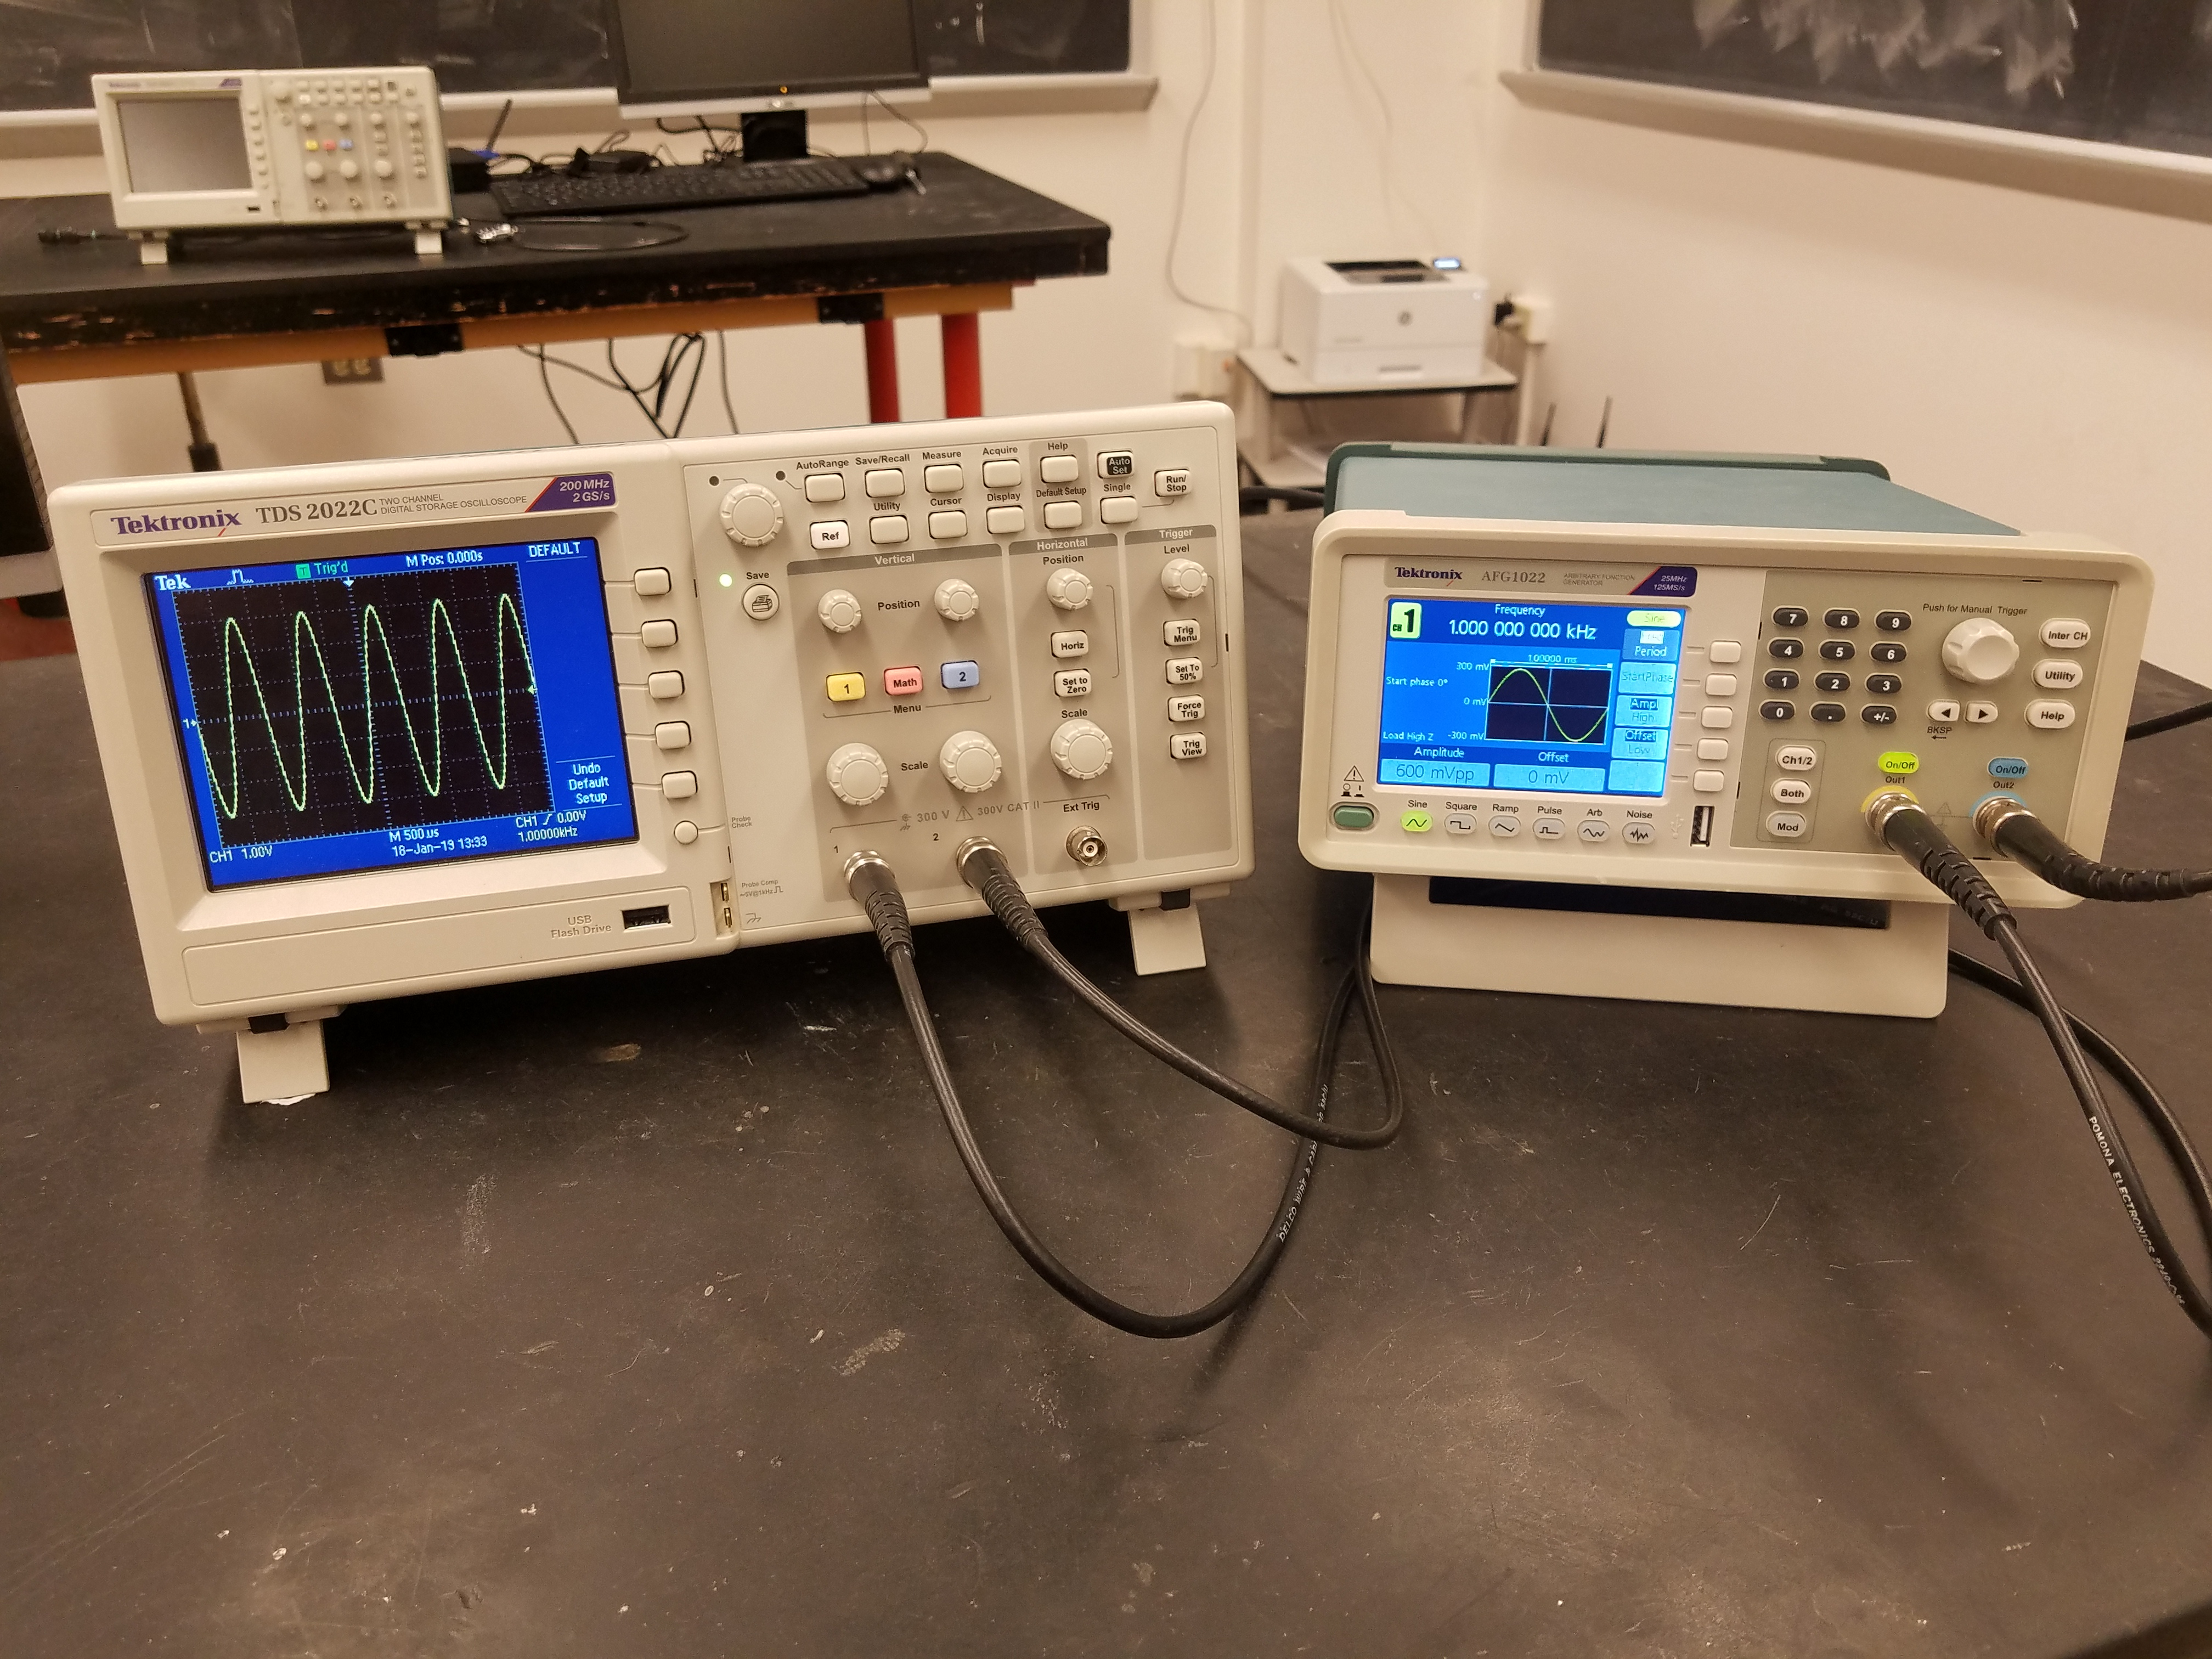
\includegraphics[width=0.45\textwidth]{figs/labs/lissajous/scope_setup.jpg} 
\caption{Connect the Channel 1 Output of your function generator directly to the Channel 1 input of your digital oscilloscope.}
\label{fig:scope_setup}
\end{center}
\end{figure}

Put your DMM aside.  Connect the Channel 1 output of your function
generator to the Channel 1 input of your digital oscilloscope.  Do the
same for Channel 2.  The setup is shown in Fig.~\ref{fig:scope_setup}.
Set your function generator to provide a $1~\rm kHz$ sine wave with
peak-to-peak voltage of $600~\rm mV$.  A DC offset of zero is implied
unless otherwise stated. Press the ``Default Setup'' button on your
digital scope.  You should immediately observe a sine wave on your
Digital scope just as in Fig.~\ref{fig:scope_setup}.

Press the button labeled ``Square'' on your function generator to
change the output from a Sine wave to a square wave and observe the
waveform on your scope.  Do the same for the Ramp and
Noise functions.  Then return to a Sine wave.

Press the yellow button labeled ``1'' several times.  This button
turns on and off the display of channel 1, and brings up the Channel 1
parameter menu.  Notice that the voltage scale for Channel 1 is
indicated as $1.0~V$.  This means that the difference between each
pair of consecutive horizontal lines corresponds to $1~V$.  We say
``One volt per division''.  By counting divisions, you should be able
to see that your waveform has a peak-to-peak voltage of $6~\rm V$.
Yet your function generator is set to produce $600~\rm mV = 0.6~\rm
V$.  Clearly someone is lying to us!

\begin{figure}[htbp]
\begin{center}
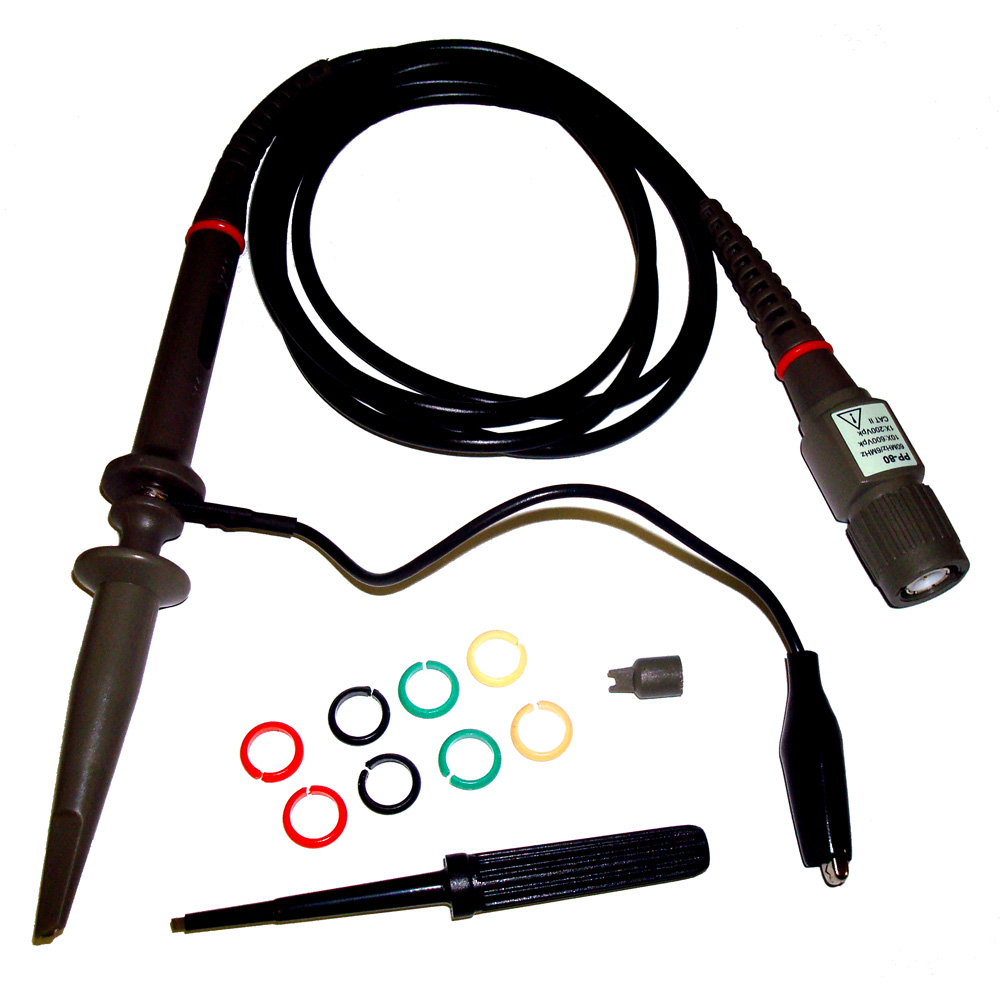
\includegraphics[width=0.45\textwidth]{figs/labs/lissajous/probe.jpg} 
\caption{An example scope probe.}
\label{fig:probe}
\end{center}
\end{figure}

Although we won't be using them in this lab, most sensitive
measurements with an oscilloscope are made using a scope probe, as
shown in Fig.~\ref{fig:probe}.  To protect the circuit being measured
from being affected by the insertion of the probe, there is usually a
large resistance in the probe.  This means that the oscilloscope
itself measures the output of a voltage divider, and the signal is
attenuated, most often by a factor of 10.  The oscilloscope simply
adjusts the voltage scale so that values you read are not attenuated.
To make consistent measurements, you simply have to make sure that the
oscilloscope is configured for the attenuation factor we are using.

In our case, we are connecting coaxial cables directly between the
oscilloscope and the function generator, and so there is no
attenuation.  But the default setup for the scope assumes that you are
using a probe with a $1/10$ attenuation, called a 10X probe.  Look at
the options next to the menu buttons and find the one that says
``Probe 10X Voltage''.  Press this menu button, and then press the
Attenuation button until it reads 1X, appropriate for a coaxial cable
with no attenuation factor.
\begin{figure}[htbp]
\begin{center}
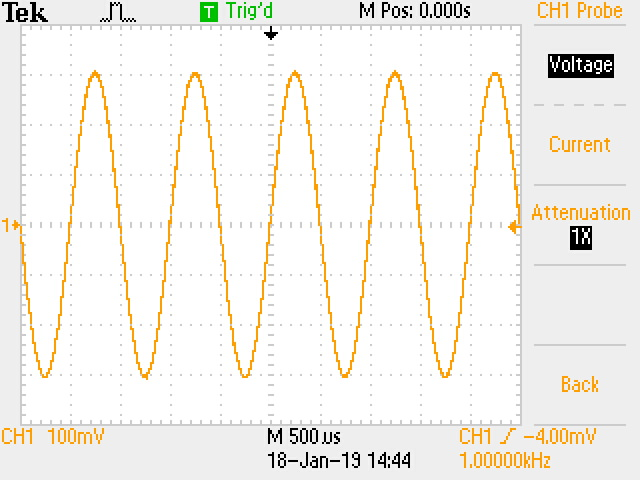
\includegraphics[width=0.45\textwidth]{figs/labs/lissajous/sine.jpg} 
\caption{Correctly scaled scope output.}
\label{fig:scopesine}
\end{center}
\end{figure}
The waveform is unchanged, but now the voltage scale is correctly set
to $100~\rm mV$.  And your signal now appears to be $600~\rm mV$,
consistent with the setting from your function generator, as shown in
Fig.~\ref{fig:scopesine}.  Next turn the knob labeled ``scale'' located
under the yellow channel ``1'' button.  Adjust this knob until the
scale for CH1 is listed as $200~\rm mV$ per division.  The apparent
size of the waveform will be reduced by a factor of two, because each
division is now $200~\rm mV$ and so your $600~\rm mV$ signal appears
three divisions high.

Next note that the function repeats every two divisions.  Since the
time scale is listed as $500~\rm \mu s$, the period is therefore $1~\rm
ms$, corresponding to a frequency of $1~\rm kHz$.  Adjust the time
scale, using the large knob in the Horizontal column, until the time
scale is $100~\rm \mu s$ per division.  This is still a $1~\rm kHz$
signal, but one period now takes up the entire display.

Using the multipurpose knob on your function generator, adjust the
frequency up to $10~\rm kHz$, and observe how the waveform changes.
Then adjust the voltage between about $100~\rm mV$ and $2~\rm V$
peak-to-peak.  When finished, leave the function generator producing a
$5~\rm kHz$ sine wave with $600~\rm mV$ peak-to-peak voltage.  Your
scope should remain at a voltage scale of $200~\rm mV$ and time scale
of $100~\rm \mu s$.  Next, set the DC offset of the signal on the
function generator by pressing:
\begin{displaymath}
{\rm Offset \to 10 \to mV}
\end{displaymath}
Turn the multipurpose knob to adjust the DC offset between $-100~\rm
mV$ and $100~\rm mV$.  Your waveform will rise and fall on your scope
display.  By default, your scope includes the DC offset, but often
this is not what you want.  On your scope, press the button labeled
``Coupling DC'', until the DC becomes AC.  When AC coupled, the DC
component of your waveform is removed.  When AC coupled, observe that
changing the DC offset on the function generator does not change the
position of the waveform.

You can adjust the position of the waveform on your scope display
using the small knobs labeled ``Position'' to adjust the offset in
vertical and horizontal.  Try this out.  To return a waveform to
(0,0), notice that the offset is displayed while you are turning the
knob.

\begin{plot}
Save a scope trace of a sine wave with a non-zero vertical and horizontal
offset. Insert your USB drive into the scope and press the Save button
(it takes few seconds to save).  Whenever you save a scope trace in
this class, make certain that there is a a date printed on the trace.
This ensures that you have your own scope traces, as they can be
confused with those from other sections.
\end{plot}

On your function generator, set the output to a $5~\rm V$ peak-to-peak
sine wave with frequency of $100~\rm kHz$.  Adjust the voltage scale
and time scale until you can clearly see the sine wave.

\section{Lissajous Figures}

\begin{figure}[htbp]
\begin{center}
\begin{tabular}{cc}
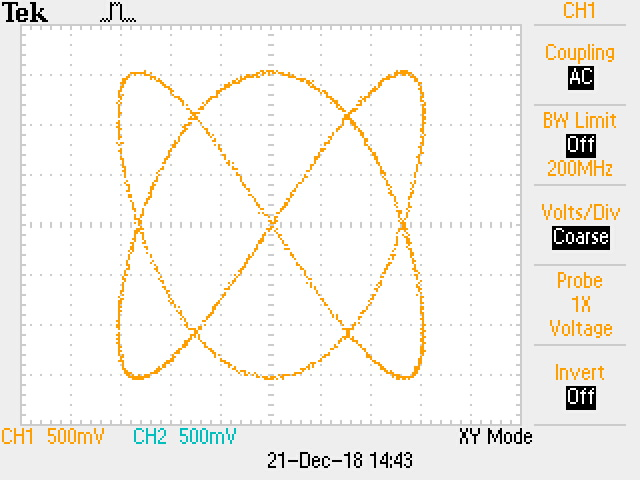
\includegraphics[width=0.45\textwidth]{figs/labs/lissajous/scope_lissajous.jpg} & 
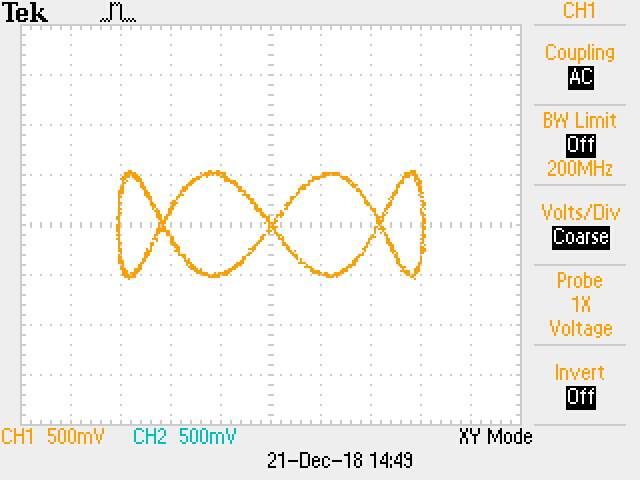
\includegraphics[width=0.45\textwidth]{figs/labs/lissajous/scope_crown.jpg} \\
(a) & (b) \\
\end{tabular}
\caption{Scope traces from Lissajous figures from settings for (a) start, and (b) crown.}
\label{fig:tracelissajous}
\end{center}
\end{figure}
Lissajous figures are the graph of system of two parameterized functions:
\begin{eqnarray*}
x &=& A_1 \sin(2 \pi f_1 t + \delta) \\
y &=& A_2 \sin(2 \pi f_2 t) 
\end{eqnarray*}
which produces a closed loop if the ratio $A_1 / A_2$ is rational.  The appearance of the figure is of a 3 dimensional knot with the viewing angle determined by the parameter $\delta$.  Two examples are shown in Fig.~\ref{fig:tracelissajous}.

To produce these figures on your scope, we'll need to use two
channels.  To begin, enable the output of both Channel 1 and Channel 2
on your function generator, and set them both to produce sine waves
with amplitude $3~\rm V$ peak-to-peak.  Adjust the frequency of
channel 1 to $2~\rm kHz$ and the channel 2 to $3~\rm kHz$.  Note that
you can switch between the Channel 1 and Channel 2 parameter menus on the function generator
with the button labeled ``Ch1/2''.

\begin{figure}[htbp]
\begin{center}
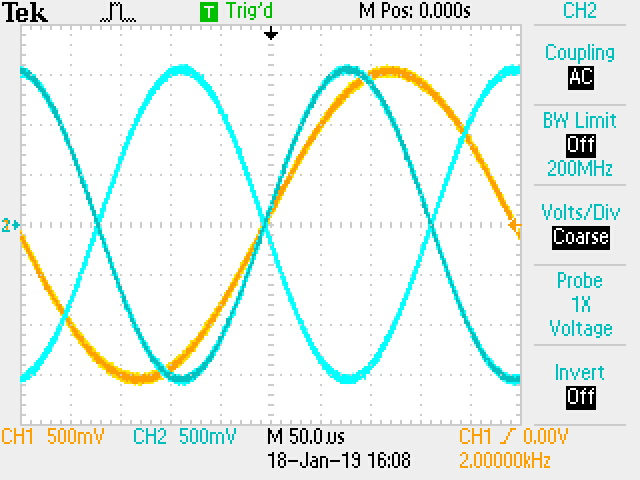
\includegraphics[width=0.45\textwidth]{figs/labs/lissajous/two_sine.jpg} 
\caption{Correctly scaled scope output.}
\label{fig:twosine}
\end{center}
\end{figure}

On your scope, switch to the Channel 2 parameter menu by pressing the
blue button labeled ``2''.  Set the coupling of Channel 2 to AC, and
probe attenuation to 1x, just as you did previously for Channel 1.
Next adjust the voltage scales of each channel to $500~\rm mV$ and set
the common time scale to something appropriate, so that you can view
both Sine waves on the scope display.  As shown in Fig.~\ref{fig:twosine},
you will see two versions of the Channel 2 output, inverted with
respect to each other, because the frequency of Channel 2 is 1.5 times
the frequency of Channel 1. You can check this but changing slightly the frequency of 
Channel 2 but return it to prescribe values to continue with the lab.

The relative phase between the two output channels of your function
generator shifts whenever you adjust the frequency of one of the
signals.  For consistent results with offline plots and the scope
traces shown here, you'll need to align the phase of the two channels
every time you adjust the frequency on the function generator:
\begin{displaymath}
\rm Inter Ch button \to AlignPhase.
\end{displaymath}

Usually, scopes are used to display the inputs as a function of time.
In this case, the voltage level is along the $y$-axis, and time is the
$x$-axis.  This mode is called YT mode.  Occasionally, however, it is
useful to display things in XY mode.  In this mode, the $x$-axis is
used for the voltage of Channel 1 and the $y$-axis is used for the
voltage of Channel 2.  Each point on the curve represents a particular
point in time.  Switch to XY mode by pressing the Display button and
then pressing the button next to the Format menu item until the mode
is XY.  You should reproduce Fig.~\ref{fig:tracelissajous}a
exactly.  If not, check that you have aligned the phase as described
above and that frequencies are set correctly as in Table.

\begin{table}
\begin{center}
\caption{Settings for various Lissajous figures.}
\label{tbl:lissajous}
\begin{tabular}{llll}
pattern & $f_1~\rm(kHz)$ & $f_2~\rm(kHz)$ & $\delta_1$ \\
start & 2 & 3 & 0 \\
fish & 2 & 3 & $135^\circ$ \\
parabola & 1 & 2 & $45^\circ$ \\
lace & 13 & 12 & 0 \\
crown & $1~\rm kHz$ & $4~\rm kHz$ & 0 \\
\end{tabular}
\end{center}
\end{table}

\begin{plot}
Adjust the phase of Channel 2, under menu item StartPhase, until the
pattern collapses into a Fish pattern (or greek letter $\alpha$) at
135 degrees.  Save a scope trace.
\end{plot}

\begin{plot}
Produce the parabola pattern according to the settings in
Table~\ref{tbl:lissajous}, saving a scope trace.  Remember to align
the phase each time you change the frequency.
\end{plot}

\begin{plot}
Produce lace pattern and save a scope trace.
\end{plot}

\begin{plot}
Produce the crown pattern, shown in Fig.~\ref{fig:tracelissajous}b.
For the right proportions, adjust the amplitude of Channel 2 to $1~\rm
V$ peak-to-peak, leaving Channel 1 at $3~\rm V$ peak-to-peak.  Notice
that as you adjust the phase of Channel 1, the crown appears to
rotate.  Adjust the frequency of Channel 2 to $4.0002~\rm kHz$.  The
crown should now appear to rotate constantly at low speed.
\end{plot}

This is a \textbf{sign-off point} for this lab. 

Please return all the components you took and cables to their
place. Leave you workstation clean.

\section{Lissajous Figures Analysis}

If you run out of time, you can finish the remaining portion of this
lab, which is exclusively done in Jupyter notebook, at another time,
such as during the Friday open lab period.  Just make sure you have
saved all of your oscilloscope traces.

Include your two scope traces in the python notebook. Make sure the
date is clearly visible on each plot. Provide a full label for each
plot which describes all the relevant information.  You can display
your scope traces in python using the Image library like this:

\begin{verbatim}
      from IPython.display import Image

       image = Image(filename='myscope.jpg') 
       display(image)
\end{verbatim}
This assumes that you copied your scope traces inside the jupyter notebook directory. 

\begin{plot} Reproduce fish pattern using scientific
python to draw the parameterized shape.  For
example, see Fig.~\ref{fig:pythonlissajous}. \end{plot}
\begin{plot} Reproduce  parabola pattern. \end{plot} 
\begin{plot} Reproduce crown pattern. \end{plot}

One way to approach this problem is to set the period to $1~\mu s$.
The functions should be evaluated at 1000 discrete times within the
interval from 0 to $1~\mu s$.
\begin{verbatim}
     t = np.linspace(0,1,num=1000)
\end{verbatim}
Define a fundamental angular frequency $\omega_0 = 2 \pi~\rm kHz$:
\begin{verbatim}
     w = 2*np.pi
\end{verbatim}
With these definitions, we would define:
\begin{verbatim}
     x = np.sin(4*w*t)
\end{verbatim}
to obtain $x$ points corresponding to $f=4~\rm kHz$ sine function.

When plotting your curves, use:
\begin{verbatim}
       plt.axis('equal')
\end{verbatim}
to keep the unit aspect ratio used by your scope.

\begin{figure}[htbp]
\begin{center}
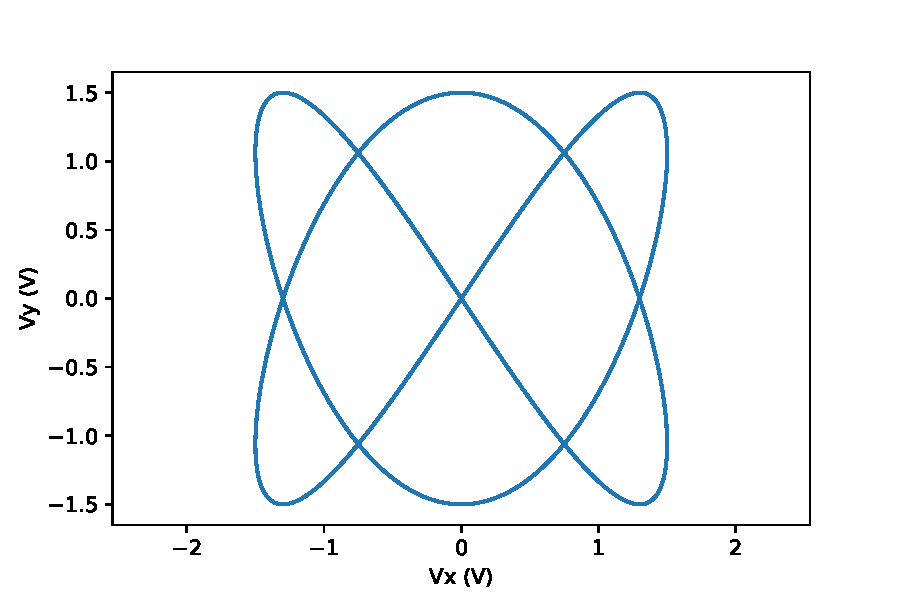
\includegraphics[width=0.45\textwidth]{figs/labs/lissajous/pythonlissajous.pdf} 
\caption{Lissajous curve constructed using Scientific Python corresponding to the scope trace in Fig.~\ref{fig:tracelissajous}a.}
\label{fig:pythonlissajous}
\end{center}
\end{figure}

\chapter{RC and RL Transient Signals}


\section{Introduction}

In this lab you will use explore transient behavior of$RC$ and $RL$ circuits.  You will learn
how to use scope probes and measure properties of waveforms on your digital oscilloscope using cursors.  For this lab there are both logbook and jupyter notebook entries.


%\section{Pre-lab Calculation}
%
%\noindent
%1) Show that for an exponential decay with time constant $\tau$, the rise-time, when defined as the time interval between $10\%$ and $90\%$ values, is given by:
%\begin{displaymath}
%t_{90} = {\rm ln}(9) \; \tau \sim 2.2 \; \tau
%\end{displaymath}
%
%\noindent
%2) Calculate the inductance of a solenoid with N=20 turns, length $\ell=4~\rm cm$, a radius of $1~\rm cm^2$ using the formula:
%\begin{displaymath}
%L = \frac{\mu_0 N^2 A}{\ell}
%\end{displaymath}
%where $A$ is the cross-sectional area and $\mu_0 = 1.257 \times 10^{-6}~\rm H/m$.


\section{Transient Response of an $RC$ Circuit}

\begin{figure}[htbp]
\begin{center}
\begin{tikzpicture}
    \node[anchor=south west,inner sep=0] (image) at (0,0,0)
         {\includegraphics[height=0.30\textheight]{figs/labs/transients/probe_setup.jpg}};
         \node[left](X) at (-1.0,4.0) {Probe Tip}; \draw (X.east) --
         (5.0,2.4); \node[left](X) at (-1.0,3.0) {Ground Clip}; \draw
         (X.east) -- (5.4,2.2); \node[right](X) at (10.0,5.0) {BNC
           Tee}; \draw (X.west) -- (8.0,5.2); \node[right](X) at
         (10.0,4.0) {Alligator pair}; \draw (X.west) -- (6.5,2.8);
\end{tikzpicture}
\caption{A setup for connecting the scope probe directly to the output of the function generator.}
\label{fig:probe_setup}
\end{center}
\end{figure}

Set your Channel 1 of your function generator to produce Square wave
output with a peak-to-peak voltage of $6~\rm V$ and a frequency of
$1~\rm kHz$.  As shown in Fig.~\ref{fig:probe_setup}, use a BNC Tee adapter
to split the output into two copies.  Send one copy directly to the
Channel 1 input of your scope.  Send the other copy to a
BNC-alligator-pair cable.  

Install an oscilloscope probe at Channel 2 of your scope (see Fig~\ref{fig:probe}).  Some probes
in the lab have the ability to switch between attenuation factors near
the probe tip.  If you have such a probe, select the 10X setting.  The
remaining probes have a fixed attenuation of 10X.

So far, we haven't had to worry about proper grounding procedure,
because this is automatically handled by the BNC cable.  Your scope
probe has two main parts, the larger probe tip, which slides to reveal
a hook which can be attached to wires and components in your circuit,
and a short lead ending with a black alligator clip called the
``Grounding clip''.  Handheld devices like your DMM have no connection
to earth ground.  The voltage reference point at the Common terminal
can be connected anywhere you would like in a circuit.  Your scope is
quite different!  It plugs into a wall outlet for power and is
referenced to earth ground.  To provide a scope which is both safe and
cost effective, most scopes are limited to making measurements which
are referenced to ground when using ordinary probes.  The ground clip
of your scope can only be connected to earth ground.  If you connect
it anywhere else in your circuit, that part of your circuit will be
short-circuited to ground.

For now, connect the probe directly to the output of the
function generator.  Your function generator is also referenced to
earth ground.  In particular for this setup, the black alligator clip
is earth ground.  Connect the black clip from the function generator
to the grounding clip for the scope probe.  Next connect the scope
probe to the red alligator clip from the function generator.  You now
have two copies of the function generator output being sent to the
scope.  One directly through the BNC cable, and one through a 10X
attenuation scope probe.

Adjust your scope to view the function generator output as measured by
Trigger 1.  Set the voltage scale as large as possible while observing
the entire wave form.  Leave the timescale at the default setting of
$500~\mu s$ for now.  Check that trigger is on the Falling edge, as set
in the last section.  Set the trigger near threshold near 0 volts.
You should observe that the position of the waveform does not vary
much with trigger threshold: the steep falling edge of the square wave
function gives us a solid reference point for defining $t=0$ in the
measurements that follow.

Now enable Channel 2 on your scope. Adjust all the necessary setting for Channel 2. It should be an identical copy of
Channel 1.  Too see both channels at the same time, you'll have to
move the vertical position of Channel 1 slightly. Closed loop tests
like this are the way experienced scientists and engineers always
start.  It allows you to setup your signal generator and scope
properly, without adding the complexity of the circuit you are working
on.  In general, avoiding confusion by taking small incremental steps
is the fastest, most reliable way to proceed in lab.  

\begin{figure}[htbp]
\begin{center}
\begin{tabular}{cc}
\begin{circuitikz}[line width=1pt]
\draw (0,0) to[square voltage source,bipoles/length=1.5cm] ++(0,4.0) to[short] ++(2.0,0)
to[R,-*] ++(0,-2.0) coordinate(X) to[short,*-o] ++(1.0,0) node[right]{A};
\draw (X) to[C,-*] ++(0,-2.0) coordinate(X) to[short,-o] ++(1.0,0) node[right]{B};
\draw (X) to[short,-*] ++(-2.0,0) node[ground,yscale=2.0]{};
\end{circuitikz}  &
\begin{circuitikz}[line width=1pt]
\draw (0,0) to[square voltage source,bipoles/length=1.5cm] ++(0,4.0) to[short] ++(2.0,0)
to[R,-*] ++(0,-2.0) coordinate(X) to[short,*-o] ++(1.0,0) node[right]{A};
\draw (X) to[L,-*] ++(0,-2.0) coordinate(X) to[short,-o] ++(1.0,0) node[right]{B};
\draw (X) to[short,-*] ++(-2.0,0) node[ground,yscale=2.0]{};
\end{circuitikz}  \\
(a) & (b) \\
\end{tabular}
\caption{A function generator driving an (a) RC circuit, and (b) RL circuit.}
\label{fig:rlc-circuits}
\end{center}
\end{figure}


Construct the circuit in Fig.~\ref{fig:rlc-circuits}a on your
breadboard, as shown in Fig.~\ref{fig:rc_setup}a.  Use $C=10~\rm nF$
capacitor and $R=10~\rm k\Omega$.  
\begin{measurement} Using the given values of resistor and capacitor, calculate and record in your logbook the time constant of the RC circuit  together with its minimum and maximum value assuming 5\% tolerance. Take care to include proper units. Using your DMM, measure and record
the actual resistance and capacitance of your components before
installing them. Record each value together with accuracy of your DMM for that specific measurement (see table~\ref{tbl:accuracy}). Then calculate the time constant of the RC circuit using the measured values. We still did not learn how to propagate uncertainties. Estimate which fractional uncertainty ($\mbox{accuracy of a value}/\mbox{measured value}$) is larger and apply this fractional uncertainty to your calculated time constant. Do the ranges for the estimates of time constant overlap? Add a comment in your logbook. \end{measurement}

 Use your function generator as the square wave
voltage source.  Recall that the black alligator clip is earth ground.
The red alligator clip is the square wave output relative to earth
ground, and corresponds to the upper terminal of the voltage source in
the diagram.  The only valid place to connect the grounding clip of
your scope probe is to earth ground, so connect that to point B in
your circuit.  Connect the scope probe tip to point A.  As shown in
the Fig.~\ref{fig:rc_setup}b, each time the square wave changes
polarity, the capacitor beings charging or discharging until it
reaches equilibrium with the new voltage, revealing the characteristic
exponential transient response.

\begin{figure}[htbp]
\begin{center}
\begin{tabular}{cc}
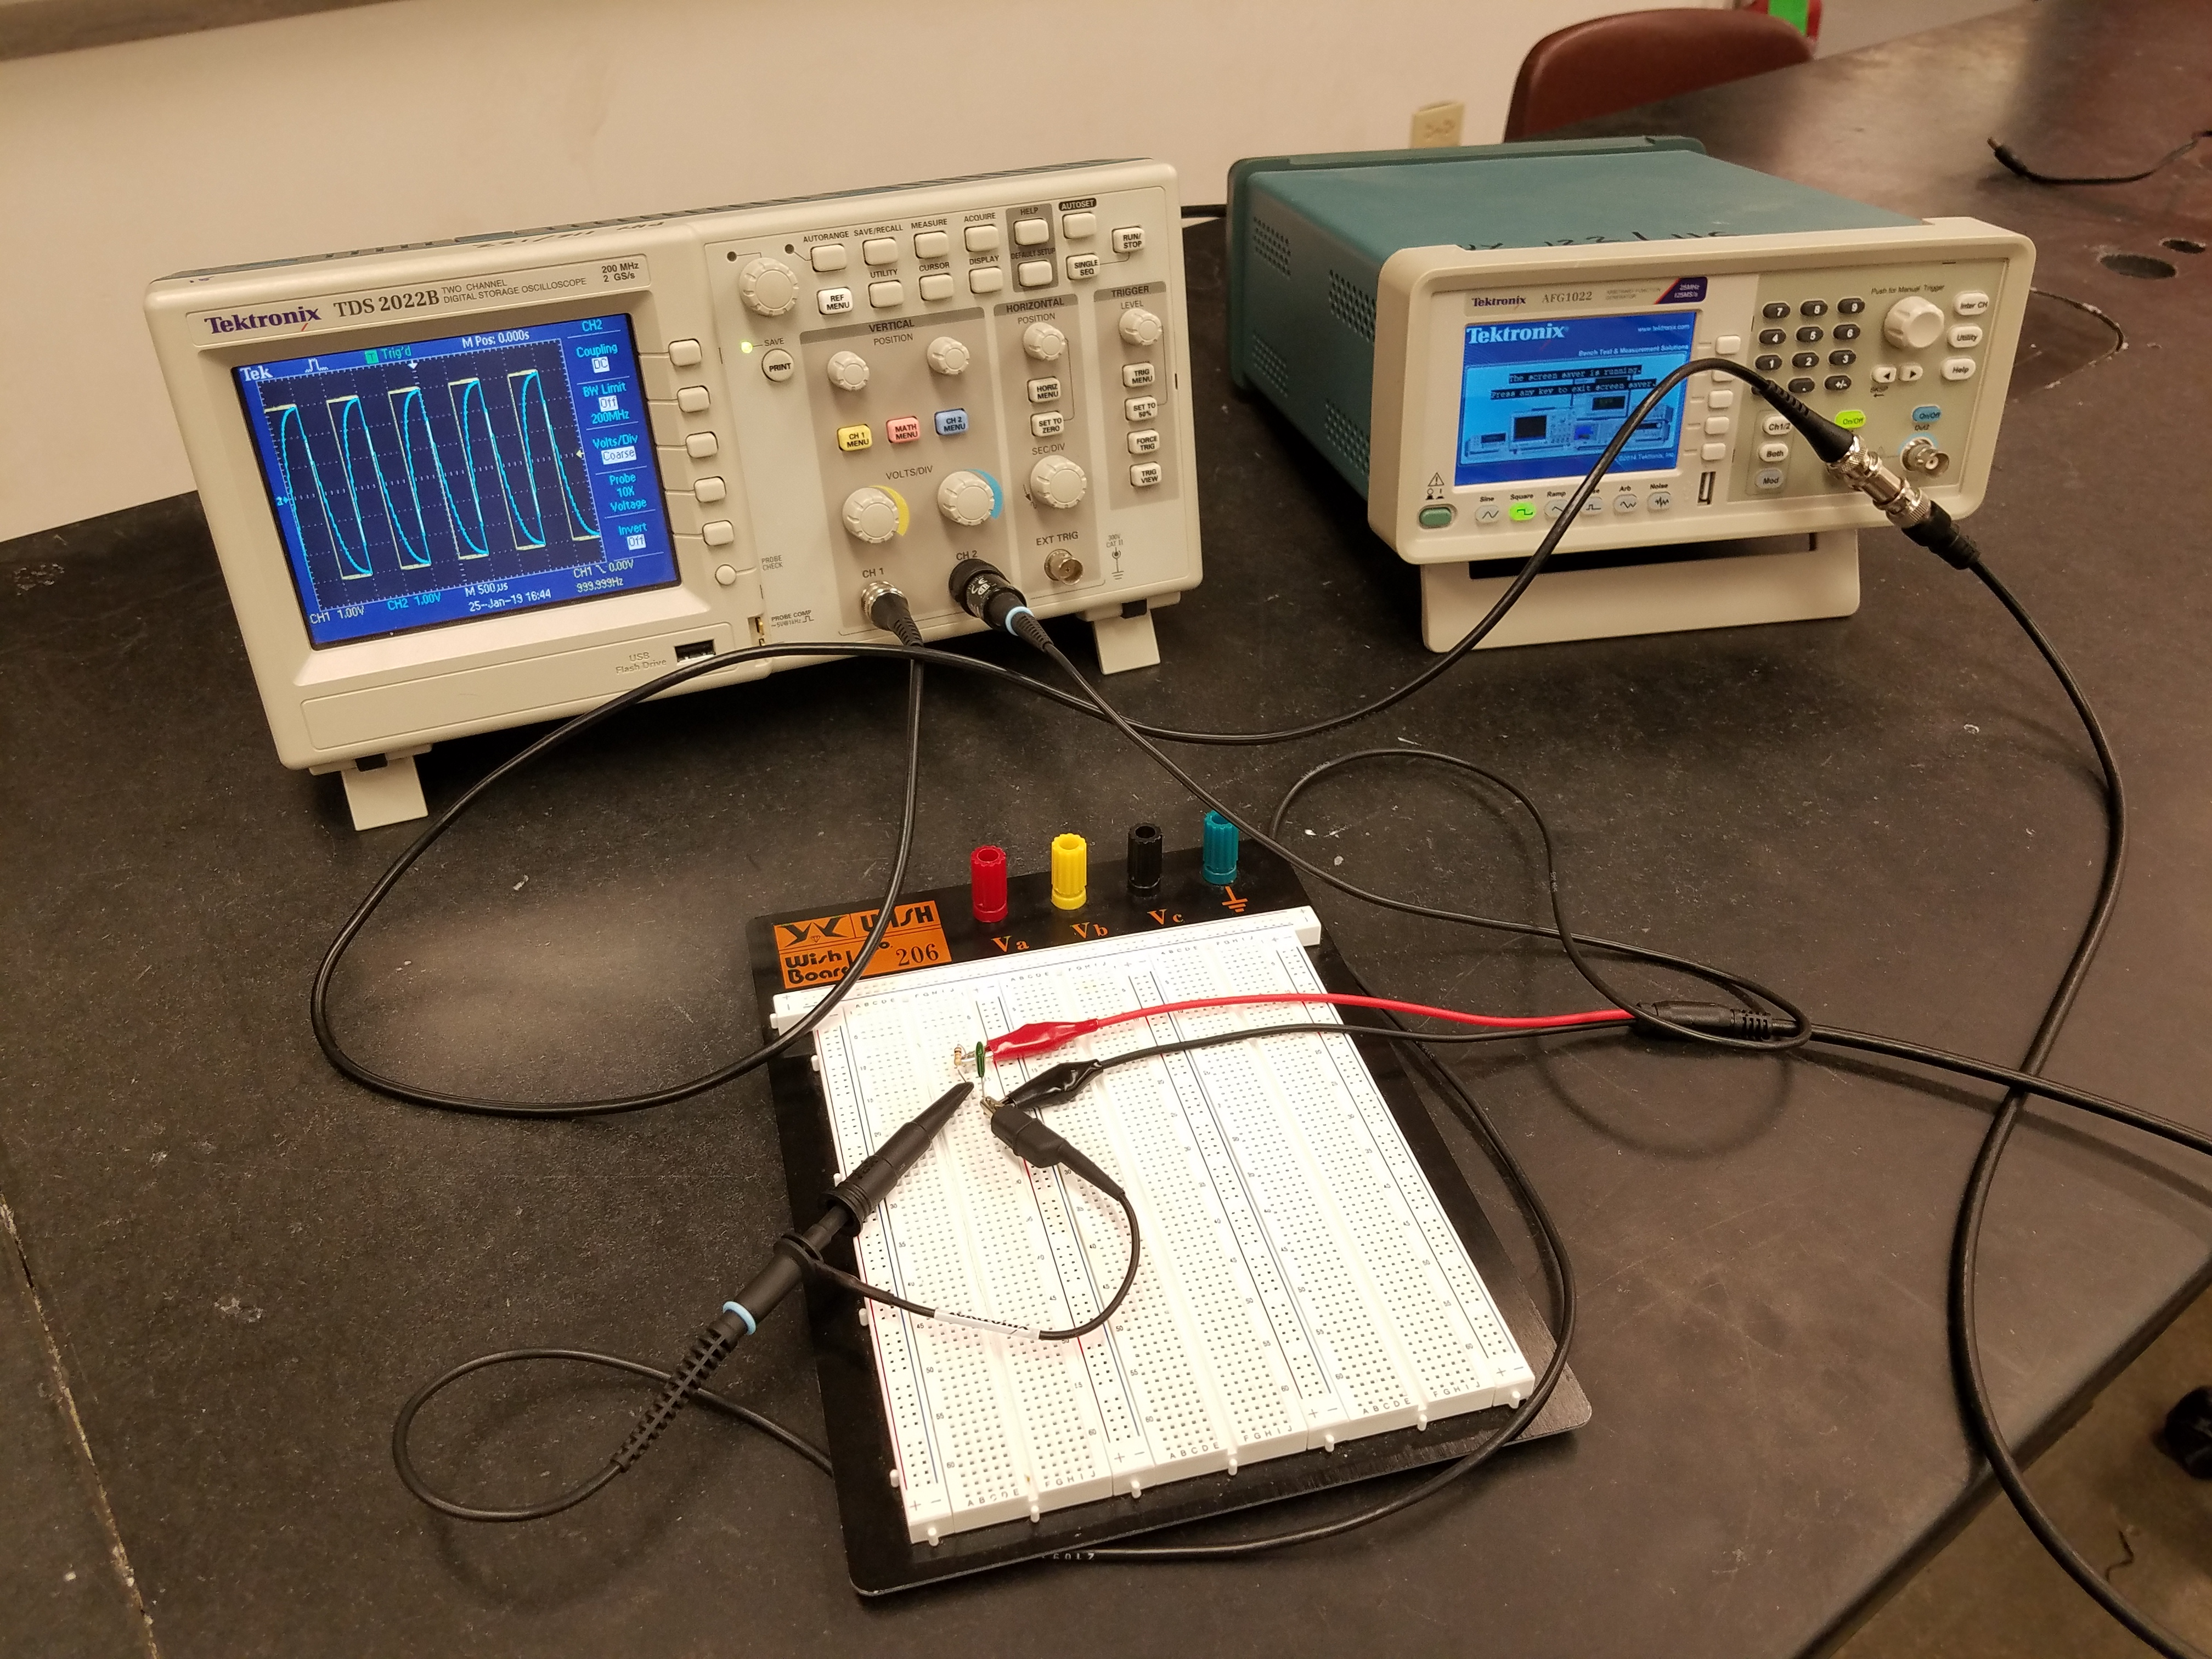
\includegraphics[width=0.45\textwidth]{figs/labs/transients/rc_setup.jpg} &
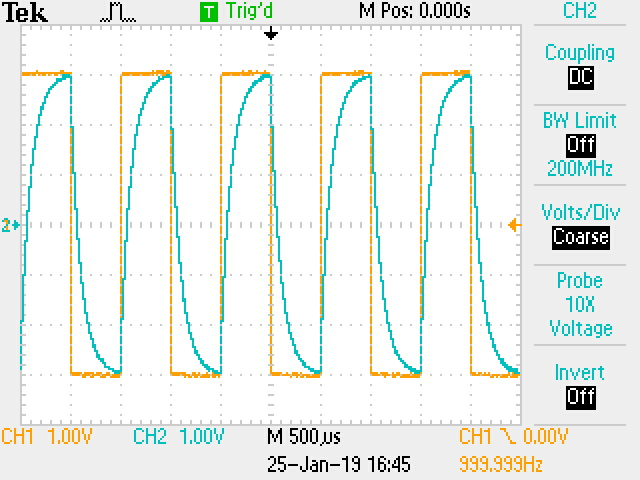
\includegraphics[width=0.45\textwidth]{figs/labs/transients/rc_trace.jpg} \\
(a) & (b) \\
\end{tabular}
\caption{Setup for the (a) RC circuit measurement, and (b) example scope trace showing exponential curve.}
\label{fig:rc_setup}
\end{center}
\end{figure}

\begin{figure}[htbp]
\begin{center}
\begin{tabular}{cc}
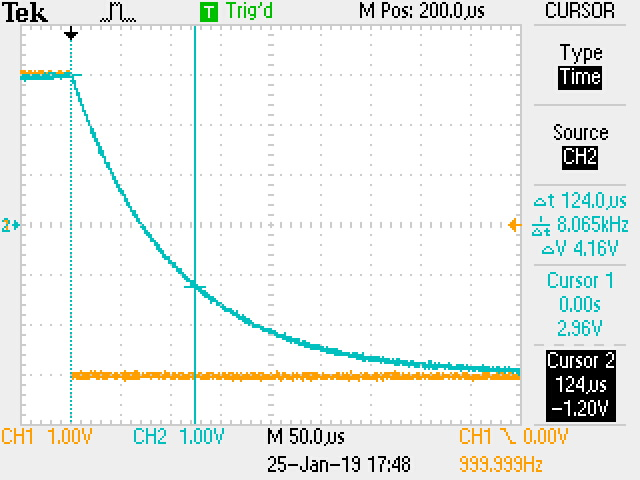
\includegraphics[width=0.45\textwidth]{figs/labs/transients/rc_cursor.jpg} &
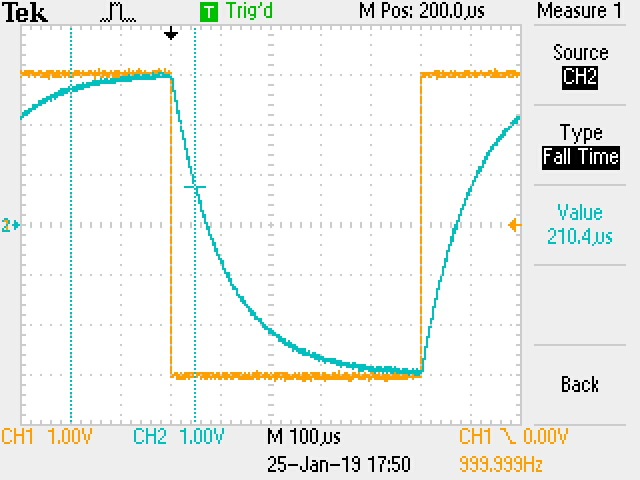
\includegraphics[width=0.45\textwidth]{figs/labs/transients/rc_falltime.jpg} \\
(a) & (b) \\
\end{tabular}
\caption{Scope traces showing (a) use of cursor to measure the waveform at $t=124~\rm \mu s$ and $V=-1.20~\rm V$, (b) use of the built in fall time measurement.}
\label{fig:cursor_falltime}
\end{center}
\end{figure}

Now adjust the timescale to zoom in on the exponential decay portion
of the curve, making sure to keep the trigger position at the left
side of the display, as shown in Fig.~\ref{fig:cursor_falltime}a.
Press the Cursor button, then set Type to Time, and Source to CH2.
This feature allows you to make measurements of different points along
the curve.  Leave Cursor 1 located at $t=0$.  Highlight Cursor 2, by
pressing the corresponding menu button, and adjust it's position using
the multipurpose knob.  Now you can make accurate measurements of the
waveform by reading off the voltage and time at anywhere that you
place the cursor.  
\begin{measurement} Record one measurement every $\sim 25~\rm \mu s$
starting from $t=0~\mu s$ to $400~\rm \mu s$.  (Recall that when
making measurements at target values, you need not hit the target
value exactly, simply record the actual position at which you made
your measurement.) Record also the sketch of your setup and the rough sketch of your waveform.\end{measurement}

\begin{measurement} Your scope can also directly measure the fall time of a waveform.
Setup the function so that one complete falling edge is on screen, as
shown in Fig.~\ref{fig:cursor_falltime}b.  Press Measure and then set
source to CH2 and Type to ``Fall Time''. You might see this value fluctuating. Record five measurements of this value in your logbook.\end{measurement}


\begin{measurement}
Show in your logbook that for an exponential decay with time constant $\tau$, the rise-time, when defined as the time interval between $10\%$ and $90\%$ values, is given by:
\begin{displaymath}
t_{90} = {\rm ln}(9) \; \tau \sim 2.2 \; \tau
\end{displaymath}
\end{measurement}

\begin{plot} Using the above relation and five measurements of fall time calculate the mean value of the time constant of the RC circuit. Recall you can use numpy functions. Calculate also the standard error of the mean value as following: $\sigma_{mean}= \mbox{standard deviation}/\sqrt{\mbox{number of measurements}}$.
\end{plot} 

\begin{measurement} Record the third estimate for the time constant of the RC circuit together with uncertainty in your logbook. Examine now all three different estimates. Are they consistent? Do the ranges for the three estimates of the time constant overlap? Add comment in your logbook about how those estimates compare to each other. Also record your qualitative understanding of this comparison. 
\end{measurement}


% Check that the measured fall time is consistent with your measured values of $R$ and $C$, using the formula from prelab. 


\section{Analysis}

\begin{plot} Plot your collected $RC$ circuit exponential decay data as discrete
data points and compare with the expected exponential decay function
as a continuous curve using the expected $RC$ time constant calculated
from: 1) given value of $R$ and $L$ (Prediction 1), 2) your measured value of $R$ and $L$ (Prediction 2) and 3) your measured value of the fall time via scope (Prediction 3).  Make sure to have
appropriate axis labels and a legend indicating ``Data'',``Prediction 1'', "Prediction 2" and "Prediction 3". 
Describe (in your jupyter notebook) how those predictions are matching your measured data? Could you tell which prediction describes your data best?
\end{plot}

\begin{plot} Redo the plot (in a new inline plot) using a log scale with base of 10 in y axis. To apply logarithmic scale explore the options for plotting in python. A logarithmic scale is a nonlinear scale often used to represent a large range of positive values. You will have to make your voltage measurements larger than zero and you can do this by shifting the measured values by a constant factor. On a logarithmic scale each increment on the axis increases by a factor of 10. On a linear scale each increment on the axis increases by equal fixed increment.  
On a linear scale, a change between two values is perceived as the difference between the values. For example, a change from 1 to 2 is the same amount of increase as from 99 to 100. On a logarithmic scale, a change between two values is perceived as the ratio of the two values. For example, a change from 1 to 2 (ratio of 1:2) is the same amount of increase as a change from 50 to 100 (also a ratio of 1:2). Describe (in your jupyter notebook) how those predictions are matching your measured data? Could you tell which prediction describes your data best? Is this plot more informative? Add these comments to your jupyter notebook. 
\end{plot}

\begin{plot} Plot a difference between data and different prediction as data points in a separate plot. This is so called residual plot. Make sure to have appropriate axis labels and a legend indicating ``Data - Prediction 1'',``Data - Prediction 2'', "Data - Prediction 3".  Recall that you will have to cast your predictions in arrays. Describe (in your jupyter notebook)  how those predictions are matching your measured data? Could you tell which prediction describes your data best? Is this plot more informative? Add these comments to your jupyter notebook. 
\end{plot}



\noindent
This is a \textbf{sign-off point} for this lab. 

\section{Transient response of an RL circuit}


\begin{measurement}
Calculate the inductance of a solenoid with N=20 turns, length $\ell=4~\rm cm$, a radius of $1~\rm cm^2$ using the formula:
\begin{displaymath}
L = \frac{\mu_0 N^2 A}{\ell}
\end{displaymath}
where $A$ is the cross-sectional area and $\mu_0 = 1.257 \times 10^{-6}~\rm H/m$.
\end{measurement}

\begin{measurement}
Wrap an inductor around the provided wooden dowel. Estimate it's
inductance by modifying your calculation above accordingly and record the value in your logbook.  Using your DMM, measure and record the actual resistance. You can skip to estimate accuracy for this measurement.
\end{measurement}


\noindent Turn down the supply to $2.5~\rm V$ peak-to-peak.  Build the circuit in
Fig.~\ref{fig:rlc-circuits}b using your homemade inductor and a
resistor of $R=47~\rm Ohms.$ 
\begin{measurement}
Measure the fall-time of your R-L circuit
and use it to determine a measured value for the inductance.
Determine and record the inductance of your coil and compare to your theoretical
estimate. Add a comment in your logbook. 
\end{measurement}

\chapter{Passive Filters}

\section{Introduction}

In this lab, you will build and measure the performance of a low-pass
and a high-pass $RC$ filter, and produce Bode plots to compare your
circuit with the impedance model derived in class and shown in
Fig.~\ref{fig:bode}.  For this lab there are both logbook and jupyter notebook entries.


\begin{figure}[htbp]
\begin{center}
%\begin{tabular}{c@{\hskip 0.25in}c}
\begin{tabular}{cc}
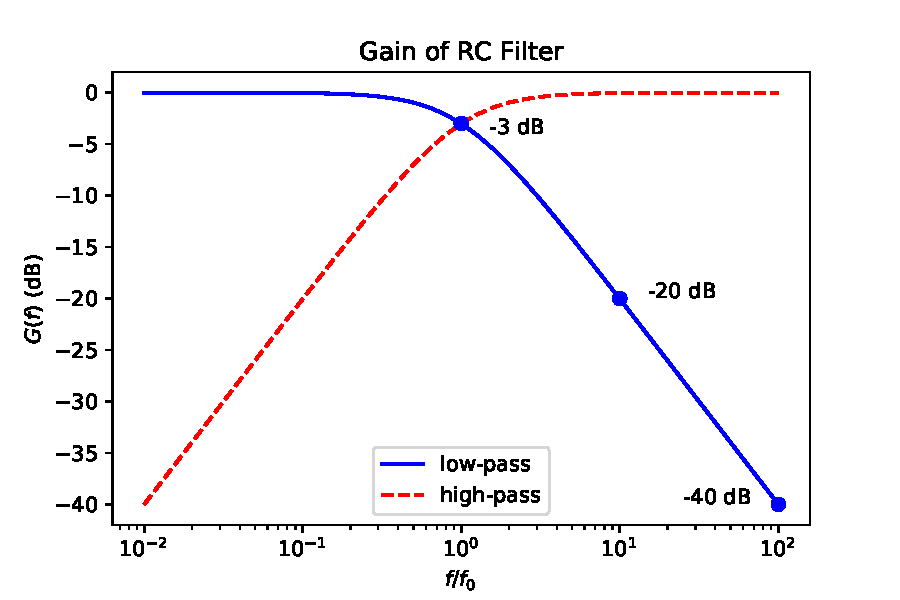
\includegraphics[height=0.22\textheight]{figs/labs/filters/rcgaindb.pdf}
&
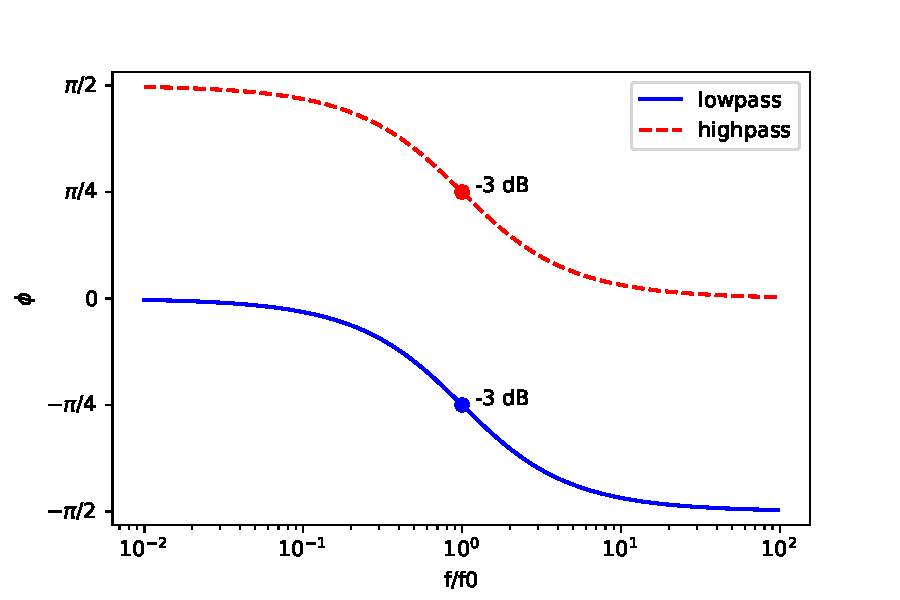
\includegraphics[height=0.22\textheight]{figs/labs/filters/rcphase.pdf} \\
(a) & (b) \\
\end{tabular}
\end{center}
\caption{\label{fig:bode} Bode plots for high-pass and low-pass filters showing the (a) gain on a dB scale, and (b) phase, both as a function of the ratio of frequency $f$ to the crossover frequency $f_0$ on a log scale.}
\end{figure}


\begin{figure}[htbp]
\begin{center}
\begin{tabular}{c@{\hskip 2cm}c}
\begin{circuitikz}[line width=1pt]
\draw (0,0) to[sinusoidal voltage source,bipoles/length=1.5cm] ++(0,4.0) to[short] ++(2.0,0) coordinate(X) to[short,*-o] ++(1.0,0) node[right]{C};
\draw (X) to[R,-*,l=$R_1$] ++(0,-2.0) coordinate(X) to[short,*-o] ++(1.0,0) node[right]{B};
\draw (X) to[C,-*,l=$C_1$] ++(0,-2.0) coordinate(X) to[short,-o] ++(1.0,0) node[right]{A};
\draw (X) to[short,-*] ++(-2.0,0) node[ground,yscale=2.0]{};
\end{circuitikz}  &
\begin{circuitikz}[line width=1pt]
\draw (0,0) to[sinusoidal voltage source,bipoles/length=1.5cm] ++(0,4.0) to[short] ++(2.0,0)coordinate(X) to[short,*-o] ++(1.0,0) node[right]{C};
\draw (X) to[C,-*,l=$C_1$] ++(0,-2.0) coordinate(X) to[short,*-o] ++(1.0,0) node[right]{B};
\draw (X) to[R,-*,l=$R_1$] ++(0,-2.0) coordinate(X) to[short,-o] ++(1.0,0) node[right]{A};
\draw (X) to[short,-*] ++(-2.0,0) node[ground,yscale=2.0]{};
\end{circuitikz}  \\
(a) & (b) \\
\end{tabular}
\caption{\label{fig:rc_circuits}
Circuit diagrams for $RC$ (a) low-pass filter and (b) high-pass filter.
The input voltage is $V_{\rm in} = V_{\rm AC}$ while the output voltage is $V_{\rm out} = V_{\rm AB}$.}
\end{center}
\end{figure}


\section{Low-pass Filters}

\begin{figure}[htbp]
\begin{center}
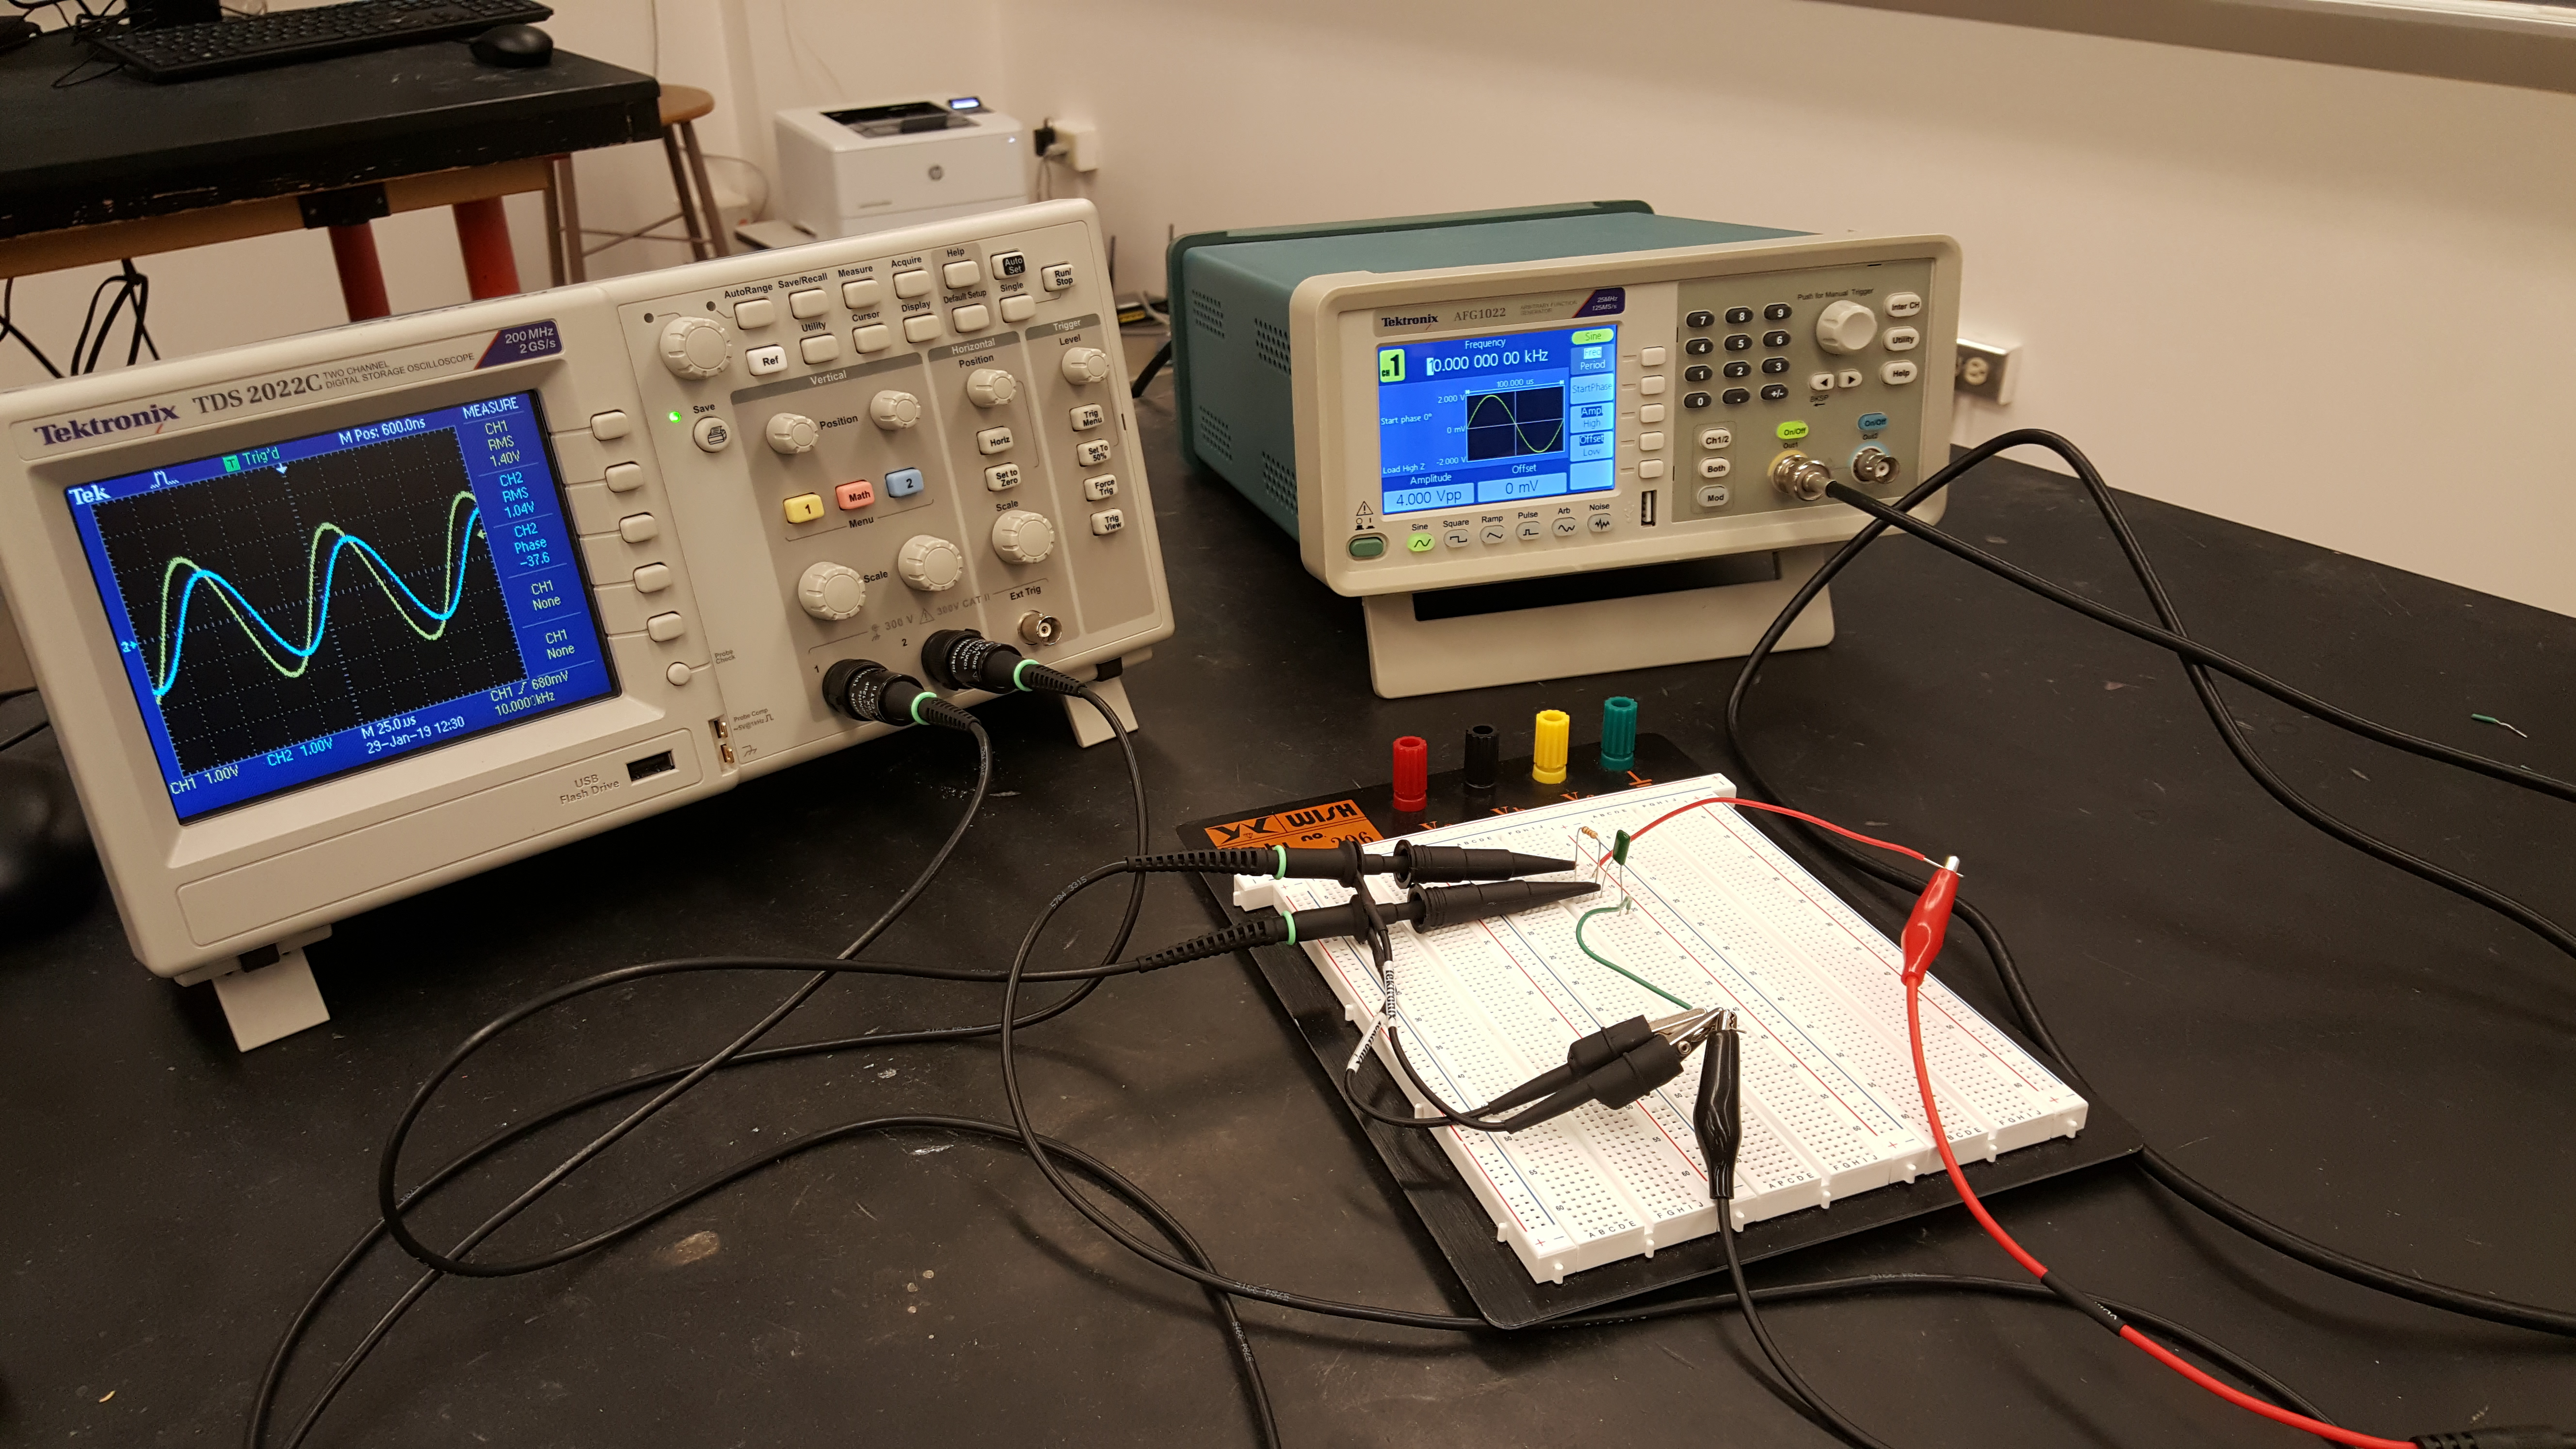
\includegraphics[height=0.22\textheight]{figs/labs/filters/filter_setup.jpg}
\end{center}
\caption{\label{fig:filter_setup} Setup for RC low-pass filter.}
\end{figure}


\begin{measurement} Calculate the corner frequency $f_0$ (aka the frequency of
$-3~\rm dB$ point) for the RC filters shown in
Fig.~\ref{fig:rc_circuits} for $R_1=1.5~\rm k\Omega$ and $C_1=10~\rm nF$.\\
\end{measurement}
\noindent Set your function generator to produce a sine function with a
peak-to-peak voltage of $4~\rm V$ and set the frequency to the calculated value of the corner frequency. %$10~\rmkHz$.  
Build the circuit shown in Fig.~\ref{fig:rc_circuits}a using
$R=1.5~\rm k \Omega$ and $C= 10~\rm nF$.  
\begin{measurement} Measure and record the
actual resistance and capacitance of the components before installing
them in your circuit. 
\end{measurement}
Use a BNC-alligator-pair cable to connect the
function generator output to your breadboard, to provide the AC
voltage source.  Keep in mind that the black alligator clip from your
function generator is earth ground, while the red alligator clip is the
function generator output referenced to ground, i.e. the top of the AC
source as drawn in the circuit diagram.

You will be using two scope probes in this lab, and as always some
care must be taken with respect to grounding when using your scope.
Your function generator has already set the earth ground point in your
circuit at the black alligator clip, which is point A in the circuit
diagram.  The scope grounding clips should both be connected to point
A.  To measure $V_{\rm in}$ on your scope Channel 1, connect the scope
probe tip of Channel 1 to point C in your circuit.  To measure $V_{\rm
  out}$ on your scope Channel 2, connect the scope probe tip of
Channel 2 to point B in your circuit.

The setup, including the scope, is illustrated in
Fig.~\ref{fig:filter_setup}.  Note in particular that the two scope
grounding clips and function generator ground are all connected to a
single (green) wire, which is used to set the ground point in the
circuit.

Set your Scope to the default setup, then adjust the timescale
appropriately and enable the output of channel 2.  
\begin{measurement} Calculate at $1\%$
precision the corner frequency $f_0$ from the measured values of your
resistor and capacitor, and set the frequency of your function
generator to that value. 
\end{measurement}

\noindent To produce the Bode plots for your filter,
we will be measuring the voltage gain $G = V_{\rm out} / V_{\rm in}$
and the phase shift $\phi$ of $V_{\rm out}(t)$ relative to $V_{\rm
  in}(t)$.

\begin{figure}[htbp]
\begin{center}
\begin{tabular}{cc}
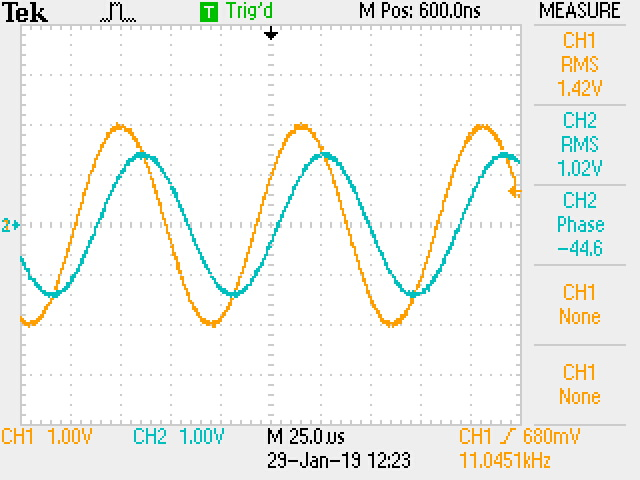
\includegraphics[width=0.4\textwidth]{figs/labs/filters/phase_measure.jpg} &
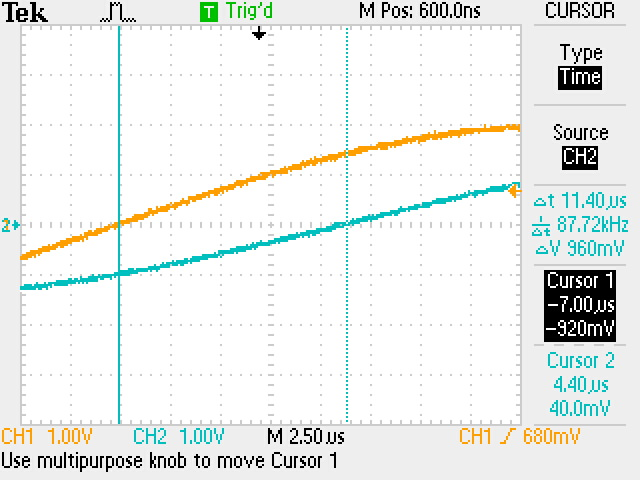
\includegraphics[width=0.4\textwidth]{figs/labs/filters/phase_cursor.jpg} \\
(a) & (b) \\
\end{tabular}
\end{center}
\caption{\label{fig:scopegain} Measuring the gain and phase with your scope.}
\end{figure}

The gain is the ratio of the amplitudes which can be read from the
scope traces.  Using the example in Fig~\ref{fig:scopegain}, the
output has an amplitude of 1.4 divisions while the input has an
amplitude of 2.0 divisions, so the gain is $G \sim 1.4/2.0 \sim
1/\sqrt{2}$.  After adjusting the horizontal scale and using the cursors menu, as
shown in Fig~\ref{fig:scopegain}, the offset in time $\Delta t$
between when each signals crosses zero is determined to be $11.4~\rm
\mu s$.  The offset in degrees is simply: 
\begin{displaymath}
\phi =  f_0 \, \Delta t \, \cdot (360^\circ).
\end{displaymath}
In this case, $\phi \sim 45^\circ$.  The phase can also be estimated
by noting that the output crosses zero half-way between where the
input crosses zero and its peak value, which is 1/8 of a period, or
$45^\circ$.  A gain of $1/\sqrt{2}$ and a phase-shift of magnitude
$45^\circ$ is expected at the cross-over frequency (or $-3~\rm dB$
point). Once you have estimated these quantities from the wave forms, you can
setup your scope to measure the appropriate quantities for you, using
the Measure menu, as shown in Fig.~\ref{fig:scopegain}.  The RMS
voltage measurement is generally the most reliable amplitude
measurement, so measure the RMS of each channel plus the phase
difference of channel 2 relative to channel 1.

\begin{measurement} 
Sketch the setup in your logbook. Measure and record the RMS amplitudes of channel 1 and channel 2, and the phase difference, at 
nine different frequencies, chosen to cover four orders of magnitude:
\begin{displaymath}
f=\{f_0/100, f_0/30, f_0/10, f_0/3,f_0, 3f_0, 10f_0, 30f_0, 100f_0\}
\end{displaymath}
where $f_0$ is the cross-over frequency.  You'll have to change the
horizontal scale appropriately as you change the frequency, as well as
the voltage scale for Channel 2 when the output is attenuated.  When
using the scopes automatic measurement functions, you should always
check at a few points by estimating the quantities yourself as shown
above.  You should note these cross-checks in your logbook. \end{measurement}

\section{High-pass Filter}

\begin{measurement} Sketch the setup in your logbook. Using the same components as in the previous section, build the
high-pass filter of Fig.~\ref{fig:rc_circuits}b, and repeat your
measurements at the nine different frequencies:
\begin{displaymath}
f=\{f_0/100, f_0/30, f_0/10, f_0/3,f_0, 3f_0, 10f_0, 30f_0, 100f_0\}
\end{displaymath}
\end{measurement}


\section{Analysis}

\begin{plot} Plot the measured gain as a function of frequency for your high-pass
and low-pass filter, and compare to the expected response (using measured values of $R$ and $C$). 
Make sure to have
appropriate axis labels and a legend indicating ``Data'',``Prediction'',.... .
Use a more descriptive wording instead of Data and Prediction (given here only as example). 
Describe (in your jupyter notebook) how those predictions are matching your measured data? \end{plot}

\begin{plot}  Plot the
measured phase shift as a function of frequency for your high-pass and
low-pass filter, and compare to the expected response. Make sure to have
appropriate axis labels and a legend indicating ``Data'',``Prediction'',.... .
Use a more descriptive wording instead of Data and Prediction (given here only as example). 
Describe (in your jupyter notebook) how those predictions are matching your measured data?
\end{plot}


\begin{plot} Plot the measured gain \textbf{in decibels} as a function of frequency for your high-pass
and low-pass filter, and compare to the expected response (using measured values of $R$ and $C$). 
Make sure to have
appropriate axis labels and a legend indicating ``Data'',``Prediction'',.... .
Use a more descriptive wording instead of Data and Prediction (given here only as example). \end{plot}

\noindent
This is a \textbf{sign-off point} for this lab. 



\chapter{Complete List of Labs}

\noindent {\bf Electron:}
\begin{enumerate}
\item DC Circuits
\item Thevenin Equivalent Circuits
\item Alternating Current and Time Varying Signals
\item RC and RL Transient Signals
\item Passive Filters and Resonance
\item The Diode
\end{enumerate}

\noindent {\bf Scientific Python Analysis Labs:}
\begin{enumerate}[resume]
\item Introduction to Plotting
\item Histograms and Distributions
\item The Central Limit Theorem
\item Error Propogation
\item Curve Fitting
\item Fourier Transforms
\item Monte Carlo Techniques
\end{enumerate}

\noindent {\bf Advanced Labs:}
\begin{enumerate}[resume]
\item Geiger Counter
\item Planck's Constant
\item Speed of Light in Cable
\item Speed of Light in\ Vacuum
\item Speed of Light Analysis
\item Muon Lifetime Analysis
\end{enumerate}

\end{document}
